\chapter{Teor\'ia funcional de la densidad} \label{cap:DFT}
	
	\section{Introducci\'on a la teor\'ia funcional de la densidad} \label{sec:introdft}
	
	La ecuaci\'on fundamental para la descripci\'on de  las propiedades de los materiales es la ecuaci\'on  de  Schr\"odinger para muchos cuerpos en donde el Hamiltoniano est\'a dada por \cite{Faustino-2014}: 
	\begin{multline}
	\hat H = - \frac{\hbar ^2}{2 m_e} \sum_{i} \nabla_{i}^2 - \sum_{i,I} \frac{Z_I e^2}{\vert \pmb{r_i} - \pmb{R_I} \vert}+ \frac{1}{2} \sum_{i \not= j}  \frac{e^2}{|\pmb{r_i} - \pmb{r_j} |}\\
	- \sum_{I} \frac{\hbar^2}{2 M_I} \nabla_I^2 + \frac{1}{2} \sum_{I \not= J} \frac{Z_I Z_J e^2}{|\pmb{R_I}-\pmb{R_J}|},  \label{ec:sh} 
	\end{multline}	
	\newline
	en donde las posiciones de los electrones en letras min\'usculas y los n\'ucleos con n\'umero at\'omico  $Z_I$, en la posici\'on $\pmb{R_I}$ y masa $M_I$ se representan con letras may\'usculas, el problema es encontrar m\'etodos para tratar con  los efectos de las interacci\'on  electr\'on-electr\'on que son fundamentales para describir los fenómenos, se observa en la ecuaci\'on \ref{ec:sh}  que no es posible resolver la ecuaci\'on de Schr\"odinger ni de forma anal\'itica ni num\'erica debido a que se tiene que resolver para una gran n\'umero de part\'iculas. Por este motivo se asume que la posiciones $\pmb{R_I}$ est\'an fijas y el \'ultimo t\'ermino de la Ec. \ref{ec:sh} es una constante que modifica la energ\'ia total de los electrones.
	\newline
	Tomando todo esto en consideraci\'on la Ec \ref{ec:sh} se puede escribir como \cite{Faustino-2014}:
	 \begin{equation}
	 \hat H = \hat T + \hat V_{ext} + \hat V_{int}+E_{II} \label{ec:shelectron}
	 \end{equation}
	cuyos t\'erminos expresados en unidades at\'omicas de Hartree ($\hbar = m_{e} = e= 4\pi / \epsilon_0 =1 $)  corresponden al operador de energ\'ia cin\'etica de los electrones $\hat T$
	\begin{equation}
	\hat{T} = \sum_{i} -\frac{1}{2} \nabla_{i}^2 ,\label{ec:shT}
	\end{equation}
	$\hat{V}_{ext}$ es el potencial entre electrones y n\'ucleo
	\begin{equation}
	\hat{V}_{ext} = \sum_{i,I} V_I (|\pmb{r_i}-\pmb{R_I}|), \label{ec:shVex}
	\end{equation}
	$\hat{V}_{int}$ es el potencial de la interacci\'on electr\'on-electr\'on
	\begin{equation}
	\hat{V}_{int} = \frac{1}{2} \sum_{i \not= j} \frac{1}{|\pmb{r_i}-\pmb{r_j}|} \label{ec:shVint}
	\end{equation}
	y el \'ultimo  t\'ermino $E_{II}$ corresponde a la constante descrita anteriormente que muestra la interacci\'on entre los n\'ucleos. La Ec. \ref{ec:shVex} es tambi\'en potencial externo con respecto a los electrones, este potencial generalmente se asume que es una interacci\'on de Coulomb aunque puede ser remplazado por un pseudopotencial que tome en cuenta los efectos de los electrones mas cercanos al n\'ucleo, tambi\'en se  pueden agregar otros "potenciales externos"  tales como campos el\'ectricos externos o de t\'erminos Zeeman para campos magn\'eticos \cite{Martin-2004}. 
	\newline
	%\newline
	\par La ecuaci\'on fundamental que gobierna un sistema cu\'antico es la ecuaci\'on de Schr\"odinger \cite{Martin-2004}
	\begin{equation}
	i \hbar \frac{d \Psi ({\pmb{r}_i}; t)}{dt} = \hat H \Psi ({\pmb{r}_i}; t), \label{ec:shtime}
	\end{equation}
	en donde $\Psi ({\pmb{r}_i}; t) \equiv \Psi ({\pmb{r}_1, \pmb{r}_2, ... ,\pmb{r}_n }; t) $ es la funci\'on de onda de muchos cuerpos. Si el Hamiltoniano (Ec.\ref{ec:sh}) no depende del tiempo entonces los eigenvalores de la Ec. \ref{ec:shtime} se pueden escribir como $ \Psi ({\pmb{r}_i}; t) =  \Psi ({\pmb{r}_i}) e^{(i E/ \hbar) t} $. El siguiente paso es tratar de aproximar este problema de muchos cuerpos a uno por lo que la  ecuaci\'on de Schr\"odinger independiente del tiempo toma la siguiente forma \cite{Martin-2004}:
	\begin{equation}
	\hat H _{eff} \Psi_{i,s} (\pmb{r}) = \left [ -\frac{\hbar^2}{2m_e} \nabla^2 + V_{eff}^{s} \right]\Psi_{i,s} (\pmb{r}) = \varepsilon_i ^{s} \Psi_{i,s} (\pmb{r}),  \label{ec:shuncuerpo}
	\end{equation}
	en donde $V_{eff}^{s}$ es el potencial de un electr\'on de spin $s$ y posici\'on $\pmb{r}$, en el estado base los electrones ocupan los eigenvalores correspondientes a menor energ\'ia obedeciendo el principio de exclusi\'on de Pauli. Conociendo que los eigenestados de la Ec. \ref{ec:shuncuerpo} son ortogonales, se puede formar una funci\'on de onda antisim\'etrica con el determinante de estos eigenestados el cual se le llama determinante de Slater \cite{Faustino-2014}, el cual tiene la siguiente forma \cite{Martin-2004}:
	\begin{equation}
	\Psi = \frac{1}{\sqrt{N !}}
	\begin{vmatrix}
	\phi_1 (\pmb{r}_1, s_1) & \phi_1 (\pmb{r}_2, s_2) & \phi_1 (\pmb{r}_3, s_3) & \cdots & \phi_1 (\pmb{r}_N, s_N) \\
	\phi_2 (\pmb{r}_1, s_1) & \phi_2 (\pmb{r}_2, s_2) & \phi_2 (\pmb{r}_3, s_3) & \cdots & \phi_2 (\pmb{r}_N, s_N)\\
	\phi_3 (\pmb{r}_1, s_1) & \phi_3 (\pmb{r}_2, s_2) & \phi_3 (\pmb{r}_3, s_3) & \cdots & \phi_3 (\pmb{r}_N, s_N) \\
	                       &  \vdots                     & \vdots                      &  \ddots & \vdots\\
	\phi_N (\pmb{r}_1, s_1) & \phi_N (\pmb{r}_2, s_2) & \phi_N (\pmb{r}_3, s_3) & \cdots & \phi_N (\pmb{r}_N, s_N) \\
	  
	\end{vmatrix} \label{ec:slater},
	\end{equation}
	en donde $\phi_i (\pmb{r}_i s_i)$ es la funci\'on de onda de un solo orbital y N es el n\'umero de electrones en el sistema.
	\newline
	Utilizando esta aproximaci\'on es posible definir expresiones que son necesarias para la teor\'ia funcional de la densidad, pudiendo definir el valor promedio con cualquier operador de la siguiente manera \cite{Martin-2004}:
	\begin{equation}
	\langle \hat{O} \rangle= \sum_{i} f_{i,s} \langle \Psi_{i,s} | \hat{O} | \Psi_{i,s}\rangle , \label{ec:prom}
	\end{equation} 
	\newline
	en donde $\langle \Psi_{i,s} | \hat{O} | \Psi_{i,s} \rangle$ es el valor de espectaci\'on del operador $\hat{O}$ y $f_{i}^{s}$ es la distribuci\'on de Fermi-Dirac, definida por:
	\begin{equation}
	f_{i}^{s}= \frac{1}{e^{\beta (\varepsilon_{i,s}-\mu)}+1}, \label{ec:fermi-dirac}
	\end{equation}
	en donde $\beta= 1/k_B T$, $\mu$ es la energ\'ia de Fermi y $\varepsilon_{i,s}$ es la energ\'ia de una part\'icula dada por $\langle \Psi_{i,s} | \hat{H} | \Psi_{i,s}\rangle$, entonces el valor promedio de la energ\'ia est\'a dado por \cite{Faustino-2014}:
	\begin{equation}
	\langle E \rangle = \langle \hat{H} \rangle = \sum_{i} f_{i,s} \langle \Psi_{i,s} | \hat{H} | \Psi_{i,s}\rangle = \sum_{i} f_{i,s}  \varepsilon_{i,s} \label{ec:energia1} .
	\end{equation}
	La siguiente simplificaci\'on que se realiza es considerar la distribuci\'on de Fermi-Dirac a una temperatura de cero grados Kelvin de tal forma que se puede aproximar como 1 para los estados por de bajo del nivel de Fermi y 0 para los restantes, utilizando esto se puede escribir la ecuaci\'on \ref{ec:energia1} como
	\begin{equation}
	E= \langle \Psi | \hat{H} | \Psi \rangle \label{ec:energia},
	\end{equation}
	en donde $\Psi$ es el determinarte de Slater (ec. \ref{ec:slater}).
	\newline
	Otra cantidad de gran importancia es la densidad, para la cual se puede definir como \cite{Martin-2004}:
	\begin{equation}
	\hat{\rho}_{s ', s}= \sum_{i} | \psi_{i,s '} \rangle n_{i,s} \langle \psi_{i,s} | \label{ec:densidad} ,
	\end{equation}
	en donde $ n_{i,s} $ es el n\'umero de ocupaci\'on para el nivel $i$ y spin $s$ y toma valores de 1 y 0 por los motivos antes mencionados. Hay que recordar que es posible reescribir la ecuaci\'on \ref{ec:prom} como $\langle \hat{O} \rangle = Tr (\hat{\rho} \hat{O} ) $, obteniéndose  una expresi\'on para la densidad \cite{Martin-2004}:
	\begin{equation}
	n_{s ', s} (\pmb{r ', r} ) = \delta_{s',s} \sum_{i} \psi_{i,s} ^{ *} (\pmb{r'}) n_{i,s} ~\psi_{i,s } (\pmb{r}) .  \label{ec:densidadr}
	\end{equation}
	Si se tiene que $\pmb{r'} = \pmb{r}  $ y $s = s '  $ se tiene una expresi\'on para la densidad electr\'onica con spin $s$:
	\begin{equation}
	n(\pmb{r})= \sum_{i} n_{i,s} | \psi_{i,s} (\pmb{r}) |^2 \label{ec:densTot}
	\end{equation}
	o en el caso de que $s \not = s '  $:
	\begin{equation}
	n_{s ', s }(\pmb{r})= \delta_{s',s} \sum_{i} \psi_{i,s '}^ {*} (\pmb{r}) n_{i,s}~ \psi_{i,s } (\pmb{r}). \label{ec:denspin}
	\end{equation}
	As\'i mismo es posible definir la densidad de magnetizaci\'on utilizando la Ec. \ref{ec:denspin} y tomando en cuenta que $s, s ' = \uparrow, \downarrow $ adem\'as de considerar solo la contribuci\'on del spin del electr\'on \cite{MB-2015}:
	\begin{equation}
	\pmb{m} (\pmb{r}) = - \mu_{B} \sum_{s,s '} \pmb{\sigma}_{s,s'}~ n_{s ', s }(\pmb{r}) , \label{ec:magn}
	\end{equation}
	en donde $\mu_B= e \hbar/2 m = 0.579 \times 10^{-4} eV~ T^{-1}$ es el magnet\'on de Borh y $ \pmb{\sigma}_{s,s'}$ es el vector formado por las matrices de Pauli; sabiendo esto es posible escribir las componentes de la ecuaci\'on \ref{ec:magn} como \cite{MB-2015}:
	\begin{subequations} \label{ec:compm}
		\begin{gather}
		m_x (\pmb{r})= -2 ~\mu_{B} ~Re~ n_{\uparrow, \downarrow} (\pmb{r}) \label{ec:compm1}\\
		m_y (\pmb{r})= -2 ~\mu_{B} ~Im~ n_{\uparrow, \downarrow} (\pmb{r}) \label{ec:compm2}\\
		m_z (\pmb{r}) = - \mu_{B} ~[n_{\uparrow, \uparrow} (\pmb{r})- n_{\downarrow, \downarrow} (\pmb{r})] . \label{ec:compm3}
		\end{gather}
	\end{subequations}
  
  Si la densidad de magnetizaci\'on est\'a dirigida solamente en la direcci\'on z, entonces se dice que es colineal, en caso contrario es no colineal. 
  \newline 
  \par En el caso de que se tenga una configuraci\'on colineal, las funciones de los orbitales de la ecuaci\'on \ref{ec:slater} se pueden representar como el producto de una funci\'on que depende de la posici\'on $ \psi_{i,s} (\pmb{r_j}) $ y otra que dependa del spin $s$, $ \alpha_i (s_j)$ \cite{Martin-2004}; adem\'as estas funciones son ortonormales y es posible obtener una nueva expresi\'on para la energ\'ia total :
  \begin{multline}
  E =\sum_{i,s} \int d\pmb{r} \psi_{i,s}^* (\pmb{r})\left [ -~\frac{1}{2} \nabla^2 + V_{ext} (\pmb{r}) \right] \psi_{i,s} (\pmb{r}) +E_{II}\\
  +\frac{1}{2} \sum_{i,j,s_i,s_j} \int d\pmb{r} d\pmb{r'} \psi_{i,s_i}^* (\pmb{r}) \psi_{j,s_j}^* (\pmb{r '}) \frac{1}{|\pmb{r}-\pmb{r'}|} \psi_{i,s_i} (\pmb{r}) \psi_{j,s_j} (\pmb{r '})\\
  -\frac{1}{2} \sum_{i,j,s} \int d\pmb{r} d\pmb{r'} \psi_{i,s}^* (\pmb{r}) \psi_{j,s}^* (\pmb{r '}) \frac{1}{|\pmb{r}-\pmb{r'}|} \psi_{j,s} (\pmb{r}) \psi_{i,s} (\pmb{r '}). \label{ec:ecEnergia}
  \end{multline} 
  El primer t\'ermino engloba la suma de los valores de expectaci\'on  de energ\'ias de un cuerpo, el tercer y cuarto terminos representan la interacci\'on directa y de intercambio entre electrones. En este caso no se hace la desestimaci\'on de la auto interacci\'on ($ i=j$) debido a que se cancela por la resta del tercer y cuarto t\'erminos, en el caso de la interacci\'on directa esta se relaciona con la energ\'ia de Hartree, la cual es una energ\'ia de auto interacci\'on  de la densidad descrita por la ecuaci\'on \ref{ec:densTot} y tratada como una densidad de carga cl\'asica \cite{Faustino-2014}:
  \begin{equation}
  E_{Hartree} = \int d \pmb{r} d \pmb{r'} \frac{n(\pmb{r}) n(\pmb{r'})}{|\pmb{r}-\pmb{r'}|} \label{ec:Hartree}.
  \end{equation}
  \newline
  Minimizando la energ\'ia del sistema (Ec. \ref{ec:ecEnergia}) utilizando los multiplicadores de Lagrange con la  restricci\'on de que las funciones de onda son ortonormales se obtienen las ecuaciones de Hartree-Fock \cite{Jo-Ko2006}:
  \begin{multline}
  \left[ -~\frac{1}{2} \nabla^2+ V_{ext} (\pmb{r})+ \sum_{j,s_j} \int d \pmb{r'} \psi_{j,s_j}^* (\pmb{r'}) \psi_{j,s_j} (\pmb{r'}) \frac{1}{|\pmb{r} - \pmb{r'}|}  \right] \psi_{i,s} (\pmb{r}) \\
  - \sum_{j} \int d \pmb{r'} \psi_{j,s}^* (\pmb{r'}) \psi_{i,s} (\pmb{r'}) \frac{1}{|\pmb{r} - \pmb{r'}|} \psi_{j,s} (\pmb{r}) = \varepsilon_{i,s} \psi_{i,s} (\pmb{r}). \label{ec:hartree_fock}
  \end{multline} 
  Este sistema de  ecuaciones se puede  escribir de forma an\'aloga a la Ec. \ref{ec:shuncuerpo} si el \'ultimo elemento correspondiente al potencial de intercambio se multiplica y divide por $\psi_{i,s }$ de tal forma que se obtiene la siguiente expresi\'on para el potencial efectivo  \cite{Martin-2004}:
  \begin{equation}
  V_{eff}^{i,s}(\pmb{r}) =V_{ext}(\pmb{r})+ V_{Hartre} (\pmb{r}) + V_{x}^{i,s} (\pmb{r}) \label{ec:poteff},
  \end{equation}
  con el potencial de intercambio $ V_{x}^{i,s} (\pmb{r}) $ definido por \cite{Martin-2004}
  \begin{equation}
  V_{x}^{i,s} (\pmb{r}) = - \sum_{j} \int d \pmb{r'} \psi_{j,s} (\pmb{r'}) \psi_{i,s} (\pmb{r'}) \frac{1}{|\pmb{r}- \pmb{r'}|} \frac{\psi_{j,s} (\pmb{r})}{\psi_{i,s} (\pmb{r})}, \label{ec:vx}
  \end{equation}
  el cual se puede describir como un potencial  de Coulomb provocado por el intercambio de la densidad de carga de un nivel j a un nivel i, representado por $ \sum_{j} \psi_{j,s} (\pmb{r'}) \psi_{i,s} (\pmb{r'}) $.
  \newline
  \par El significado de los eigenvalores de la ecuaci\'on \ref{ec:hartree_fock} est\'a dado por el teorema de Koopmans, el cual dice que se relaciona con la adici\'on o remoci\'on  de electrones para los niveles vac\'ios o llenos, respectivamente \cite{MB-2015,Koopmn-1934}.
  \newline %\newline
  \par El principal problema con la teor\'ia de Hartree-Fock es que no toma en cuenta los efectos de correlaci\'on entre los electrones y es por esta raz\'on que es importante definir la matriz de densidad   de dos part\'iculas \cite{MB-2015}:
  \begin{multline}
  n(\pmb{r},s; \pmb{r'},s' )= \left\langle \sum_{I \not= J} \delta (\pmb{r}- \pmb{r_i}) \delta (s-s_i) (\pmb{r'}- \pmb{r_j}) \delta (s'-s_i) )  \right\rangle \\
  = N(N-1) \sum_{s_3,s_4,...} \int d \pmb{r}_3 \cdots d \pmb{r}_N |\Psi (\pmb{r},s; \pmb{r'},s'; \pmb{r}_3,s_3; ..., \pmb{r}_N,s_N)|^2   \label{ec:joindensity},
  \end{multline}
  en donde $\Psi$ est\'a normalizado. Para part\'iculas que no est\'an correlacionadas, la probabilidad descrita por la ecuaci\'on \ref{ec:joindensity} es igual a la multiplicaci\'on de las probabilidades de las part\'iculas individuales, entonces una medici\'on de la correlaci\'on es $\Delta n(\pmb{r},s; \pmb{r'},s' )= n(\pmb{r},s; \pmb{r'},s' ) -n(\pmb{r},s) n( \pmb{r'},s' )$ de tal forma que se puede decir que:
  \begin{equation}
  n(\pmb{r},s; \pmb{r'},s' )= n(\pmb{r},s) n( \pmb{r'},s' ) + \Delta n(\pmb{r},s; \pmb{r'},s' ). \label{ec:def2joinprob} 
  \end{equation}
  Es conveniente definir una funci\'on de correlaci\'on de pares \cite{MB-2015}:
  \begin{equation}
  g_{s,s'} (\pmb{r},\pmb{r'})= \frac{n(\pmb{r},s; \pmb{r'},s' )}{n(\pmb{r},s) n( \pmb{r'},s' )} = 1+ \frac{\Delta n(\pmb{r},s; \pmb{r'},s' )}{n(\pmb{r},s) n( \pmb{r'},s' )} \label{ec:paircorr}
  \end{equation} 
  de tal forma que para electrones que no est\'an correlacionados, $g_{s,s'}=1$. Dicha funci\'on de correlaci\'on determina propiedades importantes en un sistema de electrones que interaccionan entre si; en particular afecta la energ\'ia del sistema. Adem\'as de la repulsi\'on cl\'asica entre electrones la ecuaci\'on \ref{ec:paircorr}, contiene tambi\'en la repulsi\'on estad\'istica de electrones de tal forma que se cumpla  el principio de exclusi\'on de Pauli. Dicho efecto es descrito principalmente por el intercambio de part\'iculas, aunque existen otros efectos cu\'anticos que est\'an incluidos en el fen\'omeno de la correlaci\'on. En resumen, la ecuaci\'on \ref{ec:paircorr} representa la probabilidad de encontrar un electr\'on con un spin $s$ en $\pmb{r}$ dado que hay otro en  $\pmb{r'}$ con spin $s'$ y se puede definir la energ\'ia de intercambio y correlaci\'on como \cite{MB-2015}:
  \begin{equation}
  E_{XC} = \frac{1}{2} \sum_{s,s '} \int d \pmb{r} d \pmb{r'} \frac{1}{|\pmb{r}- \pmb{r'}|} n_{s,s} (\pmb{r}) n_{s',s'} (\pmb{r'}) [g_{s,s'} (\pmb{r}, \pmb{r'})-1]. \label{ec:energiaXC}
  \end{equation} 
  Esta energ\'ia caracteriza los efectos no cl\'asicos de la interacci\'on  electr\'on-electr\'on en la energ\'ia total. Una vez que se conoce de forma exacta  la funci\'on de correlaci\'on de pares (Ec. \ref{ec:paircorr}) entonces se tiene la enrg\'ia total del sistema.
  \section{Teoremas de Hohenberg-Kohn} \label{sec:Ho-Ko}
  Como se ha dicho en la secci\'on anterior, el problema fundamental en la descripci\'on de  las propiedades de los materiales consiste en resolver la Ec.  \ref{ec:shtime} y utilizando el Hamiltoniano de un sistema de muchos cuerpos (Ec. \ref{ec:sh}), siendo el problema muy complicado por lo que es necesario realizar aproximaciones, tales como no considerar el movimiento de los iones y realizando una aproximaci\'on a un problema de un solo cuerpo (Ec. \ref{ec:shuncuerpo}). Utilizando la teor\'ia de Hartree-Fock se encuentra que el funcional de la energ\'ia est\'a dado por la ecuaci\'on \ref{ec:ecEnergia} aunque aun existen 3N grados de libertad lo cual har\'ia imposible la resoluci\'on del problema. La siguiente aproximaci\'on consiste en expresar el funcional de la Ec. \ref{ec:energia} en funci\'on de la densidad electr\'onica para tener solamente 3 grados de libertad. Dicha aproximaci\'on implica  sustituir las interacciones individuales de los cuerpos por una sola, en donde el ensamble de electrones es representado por su densidad y \'esta es la base de la teor\'ia funcional de la densidad (DFT) la cual se ilustra en la figura \ref{im:dftIdea} \cite{MB-2015}.
  \begin{figure}[!hbt]
  	\centering
  	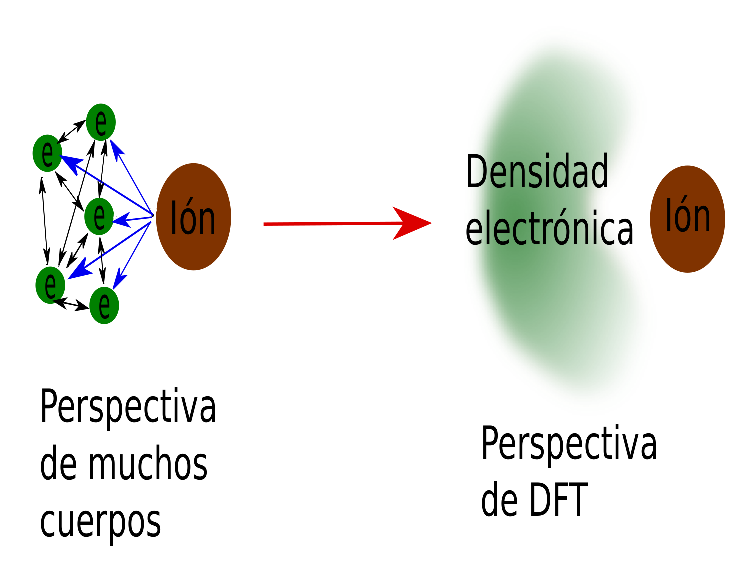
\includegraphics[width=7.0cm,height=7.0cm]{figuras/perspectivaDFT.eps}
  	\caption[Perspectiva de la teor\'ia Funcional de la Densidad.]{Idea de la Teor\'ia Funcional de la Densidad que consiste en sustituir las interacciones de muchos cuerpos con una interacci\'on promedio por medio de una densidad electr\'onica. \cite{MB-2015}}
  	\label{im:dftIdea}
  \end{figure}
  
  La teor\'ia desarrollada por Hohenberg y Kohn \cite{HK-1964} para una formulaci\'on de DFT como una teor\'ia exacta de un sistema de muchos cuerpos  solo es v\'alida para su estado base por lo tanto  es importante encontrar los valores de expectaci\'on en funci\'on los estados base $\Psi_0$ para la energ\'ia, la densidad electr\'onica y la  magnetizaci\'on  (Ecs. \ref{ec:energia}, \ref{ec:denspin} y \ref{ec:magn}, respectivamente). Es importante separar el Hamiltoniano  de la ecuaci\'on \ref{ec:shelectron} como:
  \begin{equation}
  \hat{H} =\hat{H}_0 + \hat{H}_{ext}, \label{ec:sepHamilton}
  \end{equation}
  en donde $\hat{H}_0 = \hat{T}+\hat{V}_{int}$ y $\hat{H}_{ext}= \hat{V}_{ext} + E_{II}$.  Cuando se desea considerar el aporte de la magnetizaci\'on es necesario agregar una interacci\'on de estilo Zeeman de un campo magn\'etico externo 
  $-\pmb{B}_{ext} (\pmb{r}) \cdot \pmb{m} (\pmb{r}).$\cite{Martin-2004} 
  Este potencial es valido debido a que solo se considera el aporte de la magnetizaci\'on del spin y se puede considerar el potencial de interacci\'on debido a fuentes externas \cite{MB-2015, Martin-2004} como 
  \begin{equation}
  \hat{H}_{ext} = \hat{V}_{Ex}^{s', s} = \hat{V}_{ext} \delta_{s',s} - \pmb{B}_{ext} (\pmb{r})\cdot \pmb{m} (\pmb{r}) +E_{II}. \label{ec:intExt}
  \end{equation}
  En caso de que se trabaje con una orientaci\'on no colineal, es necesario agregar el t\'ermino de acople spin-\'orbita al campo magn\'etico externo \cite{MB-2015}:
  \begin{equation}
  \pmb{B}_{ext} (\pmb{r}) \to  \pmb{B}_{ext} (\pmb{r}) + \frac{i \hbar^2}{\mu_{B} (2 m c)^2} \{[\nabla V_{ext}]\times \nabla \}.
  \label{ec:Spinorb}\end{equation}
  \newline
  La teor\'ia desarrollada muestra que el funcional de la energ\'ia est\'a caracterizado por la densidad de electrones (Ec. \ref{ec:densidadr}) y la magnetizaci\'on (Ec. \ref{ec:magn}) \cite{PhysRevB.37.10685}:
  \begin{equation}
  E=E_{V_{ext}, \pmb{B}_{ext}} [n,\pmb{m}]. \label{ec:func1}
  \end{equation}
\newline
  \par El primer teorema de Hohenberg y Kohn se relaciona con el hecho  de que el potencial externo dado por la Ec. \ref{ec:intExt}  est\'a determinado \'unicamente por la densidad y la magnetizaci\'on en el estado base $n_0$ y $\pmb{m}_0$. Esto se muestra en la figura \ref{fig:hk1},   en donde las flechas azules muestran la soluci\'on que usualmente se sigue para resolver la ecuaci\'on de Schrödinger y la flecha roja indica la relaci\'on establecida por el primer teorema de Hohenberg-Kohn.  Como consecuencia de este teorema dos estados base distintos $\Psi_0 $ y $\Psi_0 '$ dan lugar a dos matrices de densidad de spines diferentes $n_{s',s} \not =n_{s',s}' $ y por lo tanto $n(\pmb{r}), \pmb{m}(\pmb{r}) \not = n'(\pmb{r}), \pmb{m}'(\pmb{r})$. Debido a este teorema es posible determinar las funciones de muchos cuerpos para todos los niveles sin importar que est\'en desocupados y entonces todas las propiedades del sistema se pueden determinar teniendo s\'olo la densidad de electrones en el estado base \cite{HK-1964, PhysRevB.37.10685}.
  \begin{figure}[!hbt]
  	\centering
  	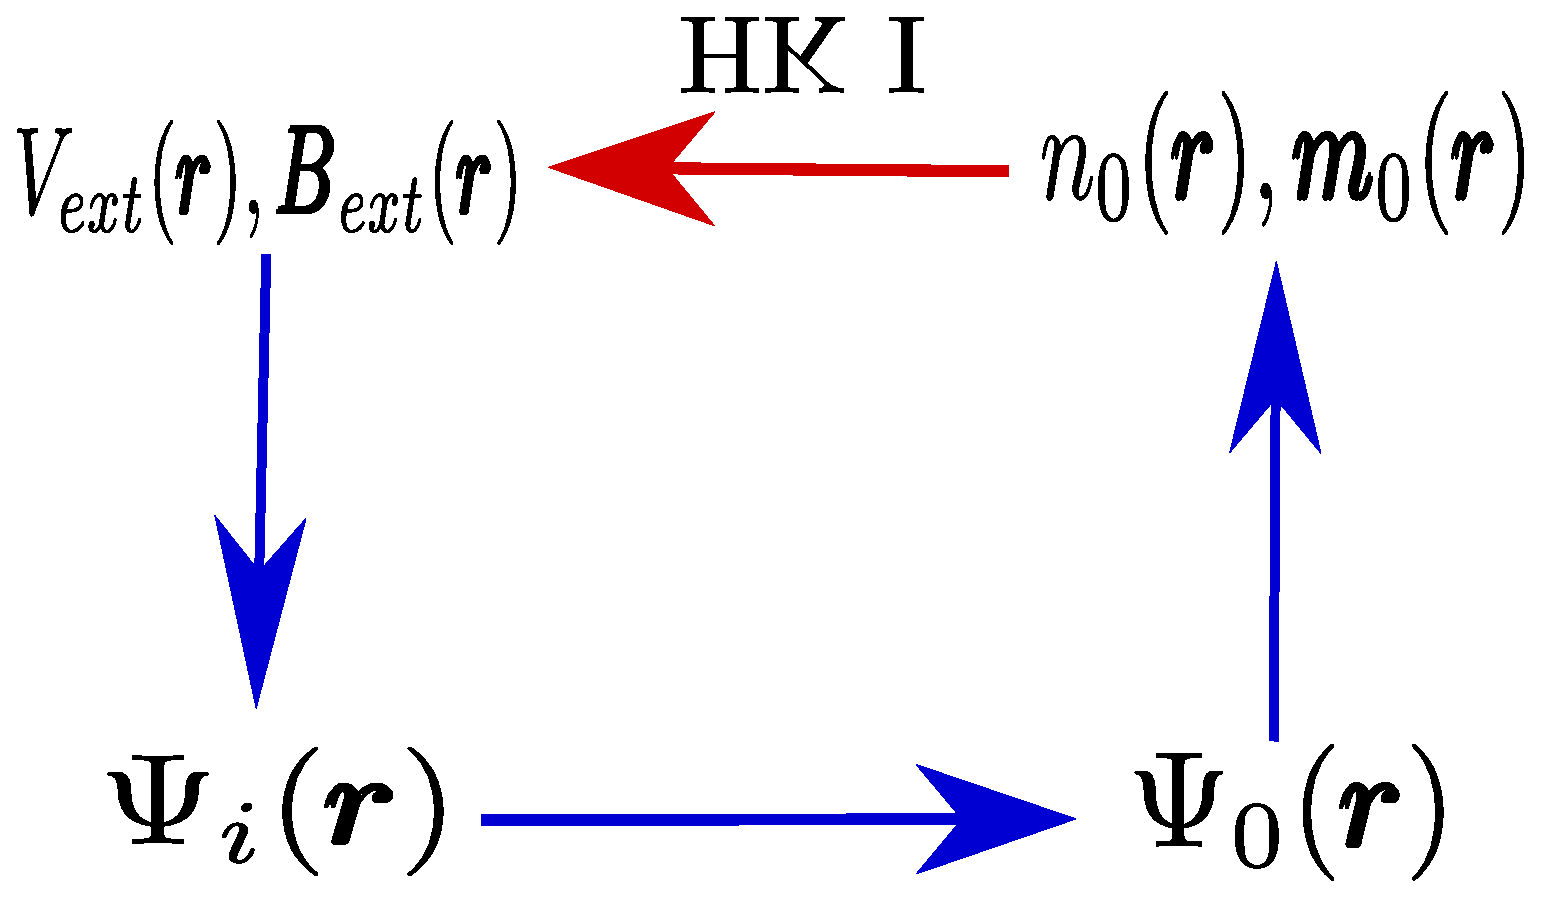
\epsfig{file=figuras/HK1.eps, width=8.0cm,height=5.0cm}
  	\caption[Primer teorema de Hohenberg-Kohn]{Representaci\'on esquem\'atica del primer teorema de Hohenberg-Kohn}
  	\label{fig:hk1}
  \end{figure}


%  \newline
  \par El segundo teorema esta relacionado con la posibilidad de determinar un funcional para la energ\'ia $E_{V_{ext}, \pmb{B}_{ext}}[n,\pmb{m}]$ en t\'erminos de la densidad y la magnetizaci\'on que es v\'alido para cualquier potencial externo $\hat{V}_{Ex}^{s', s}$. Para un $\hat{V}_{Ex}^{s', s}$ particular, la energ\'ia del estado base del sistema es el m\'inimo global de este funcional y la densidad $n(\pmb{r})$ y la magnetizaci\'on $\pmb{m}(\pmb{r})$ que minimizan el funcional son los par\'ametros exactos para el estado base  $n_0(\pmb{r})$ y $\pmb{m}_0(\pmb{r})$. Este potencial se puede escribir como \cite{PhysRevB.37.10685}
  \begin{equation}
   E_{V_{ext}, \pmb{B}_{ext}}[n,\pmb{m}]= F[n,\pmb{m}] + \int d \pmb{r} \{V_{ext} (\pmb{r}) n(\pmb{r})+\pmb{B}_{ext} (\pmb{r}) \cdot \pmb{m} (\pmb{r}) \} +E_{II}, \label{ec:funcional}
  \end{equation}
  en donde$F[n,\pmb{m}]$ es el llamado funcional universal el cual incluye las energ\'ias cin\'eticas y potencial del sistema de electrones:
  \begin{eqnarray}
  F[n,\pmb{m}]&= \langle \Psi_0 [n,\pmb{m}]| \hat{T}+\hat{V}_{int} | \Psi_0 [n,\pmb{m}] \rangle \nonumber \\
              &= T[n,\pmb{m}] + V_{int} [n,\pmb{m}]. \label{ec:funcF}
  \end{eqnarray}
  
  Si se considera  la densidad $n_0 (\pmb{r})$ y la magnetizaci\'on $\pmb{m}_0  (\pmb{r})$ del estado base, se puede determinar la energ\'ia
  \begin{equation}
  E_0= E_{V_{ext}, \pmb{B}_{ext}}[n_0,\pmb{m}_0], \label{ec:estadoBase}
  \end{equation}
  la cual obedece la desigualdad
  \begin{equation}
  E_0 < E_{V_{ext}, \pmb{B}_{ext}}[n,\pmb{m}], \label{ec:desig}
  \end{equation}
  en donde $ n (\pmb{r}),\pmb{m} (\pmb{r}) \not = n_0 (\pmb{r}),\pmb{m}_0 (\pmb{r})$. Tomando esto en consideraci\'on  se puede establecer el segundo  teorema de Hohenberg-Kohn como sigue \cite{MB-2015}:
  \begin{equation}
  E_0 = \min_{n  \to n_0, \pmb{m} \to \pmb{m}_0} E_{V_{ext}, \pmb{B}_{ext}}[n,\pmb{m}]  \label{ec:HKII}.
  \end{equation}
  Por consecuencia de este segundo teorema, el funcional de la Ec. \ref{ec:funcional} es suficiente para determinar la energ\'ia del estado base as\'i como su densidad y magnetizaci\'on. En la siguiente secci\'on se mostrar\'a el proceso general para encontrar estos valores por medio de las ecuaciones de Kohn-Sham, adem\'as que se mostrar\'a la raz\'on por la que se les llama evaluaci\'on auto consistente.
  
  \section{Ecuaciones de Kohn-Sham} \label{sec:KSH}
   Las ecuaciones de Kohn-Sham representan un sistema de ecuaciones auxiliares para resolver el problema de muchos cuerpos que representa el Hamiltoniano de la Ec. \ref{ec:sh}. Estos autores propusieron que la densidad y la magnetizaci\'on del estado base pueden ser representados con un sistema auxiliar para part\'iculas sin interacci\'on, en donde el Hamiltoniano auxiliar se elige de tal forma que el operador de  energ\'ia cin\'etica $ \hat{T}$ y el potencial local $ V_{eff}^s $ act\'uan sobre un electr\'on con spin $s$ en la posici\'on $\pmb{r}$. Tal Hamiltoniano del sistema auxiliar se puede escribir como (en unidades de Hartree) \cite{Martin-2004}:
  \begin{equation}
  \hat{H}_{aux}^{s} = - \frac{1}{2} \nabla^2 + V_{eff}^s (\pmb{r}). \label{ec:HAux}
  \end{equation}  
  Si se considera un sistema de spines colineales,  el n\'umero de electrones independientes es $N = N_{\uparrow}+ N_{\downarrow}$ y la densidad de electrones en este sistema est\'a dada por la Ecuaci\'on \ref{ec:denspin} con $s' = s$ de tal forma que la energ\'ia cin\'etica de una sola part\'icula $T_{sp}$, en donde no existe ning\'un potencial, se define como \cite{MB-2015}:
  \begin{equation}
  T_{sp} = -\frac{1}{2} \sum_{s} \sum_{i} n_{i,s} \int d^3 r ~\psi_{i,s }^* (\pmb{r}) \nabla^2 \psi_{i,s } (\pmb{r})  = \frac{1}{2} \sum_{s} \sum_{i} n_{i,s} \int d^3 r  |\nabla \psi_{i,s } (\pmb{r}) |^2 .\label{ec:funCinetica}
  \end{equation}
    Por lo tanto se puede reescribir la funcional de la Ec. \ref{ec:funcional} sin considerar campos magn\'eticos externos como: 
   \begin{equation}
   E_{KS}[n] = T_{sp}[n]+ \int d \pmb{r} V_{ext} (\pmb{r}) n_s (\pmb{r}) +E_{Hartree} [n] + E_{XC}^s [n] + E_{II}. \label{ec:funcHK}
   \end{equation}
    Los efectos de intercambio y correlaci\'on se agrupan en $E_{XC}^s [n]$, el cual se puede escribir en t\'erminos del funcional de Hohenberg-Kohn (ec. \ref{ec:funcional}) \cite{Martin-2004} :
   %\begin{equation}
   %E_{XC}^s [n] = F[n]-(T_{sp} [n]+E_{Hartree}[n]) \label{ec:eXC2}
   %\end{equation}
   %la cual se puede reescribir como:
   \begin{equation}
   E_{XC}^s [n]= \langle \hat{T} \rangle - T_{sp} [n]+\langle \hat{V}_{int} \rangle-E_{Hartree} [n] \label{ec:Exc2},
   \end{equation}
    en donde se observa que la energ\'ia de intercambio y correlaci\'on no solo depende de la diferencia entre las interacciones de Coulomb ($\langle \hat{V}_{int} \rangle-E_{Hartree}[n]$), sino que tambi\'en por la diferencia entre la energ\'ia cin\'etica entre el sistema con interacciones y el que no las tiene ($ \langle \hat{T} \rangle - T_{sp} [n] $) \cite{MB-2015}.
   \newline
   \par Para cumplir con el segundo teorema de Hohenberg y Kohn, se minimiza el funcional de la energ\'ia (ec. \ref{ec:funcHK}) con respecto  a las funciones de los orbitales $\psi_{i,s } $: 
   \begin{equation}
   \frac{\delta E_{KS} [n_s]}{\delta \psi_{i,s } ^* (\pmb{r})}= \frac{\delta T_{sp} }{\delta \psi_{i,s } ^* (\pmb{r}) } + \left[\frac{\delta E_{ext}}{\delta n_s (\pmb{r})}+\frac{\delta E_{Hartree}}{\delta n_s (\pmb{r})}+  \frac{\delta E_{XC}^s}{\delta n_s (\pmb{r})}\right] \frac{\delta n_s (\pmb{r})}{\delta \psi_{i,s } ^* (\pmb{r})} =0. \label{ec:ecEulerFun}
   \end{equation}
   Utilizando las ecuaciones \ref{ec:denspin} y \ref{ec:funCinetica} se obtiene lo siguiente:
   \begin{equation}
   \frac{\delta T_{sp} }{\delta \psi_{i,s } ^* (\pmb{r}) }= -\frac{1}{2} \nabla^2 \psi_{i,s } (\pmb{r}); ~~ \frac{\delta n_s (\pmb{r})}{\delta \psi_{i,s } ^* (\pmb{r})}= \psi_{i,s } (\pmb{r}) \label{ec:simp};
   \end{equation} 
   adem\'as sustituyendo  la Ec. \ref{ec:simp} en \ref{ec:ecEulerFun}    y utilizando el m\'etodo de los multiplicadores de Lagrange  sujeto a la condici\'on $\langle \psi_{i,s} | \psi_{j,s'} \rangle =   \delta_{i,j}\delta_{s',s}$,   se obtiene la ecuaci\'on de Kohn-Sham:
   \begin{equation}
   (H_{KS}^s -\epsilon_{i,s})\psi_{i,s } (\pmb{r}) = 0 \label{ec:ShKS},
   \end{equation}
   en donde $ H_{KS}^s $ es el Hamiltoniano efectivo definido por \cite{PhysRev.140.A1133}:
   \begin{equation}
    H_{KS}^s = -\frac{1}{2} \nabla^2 + V_{KS}^s (\pmb{r}), \label{ec:HamiltonianoKS}
   \end{equation}
   con
   \begin{eqnarray}
     V_{KS}^s (\pmb{r}) &=& V_{ext} (\pmb{r})+  \frac{\delta E_{Hartree}}{\delta n_s (\pmb{r})}+  \frac{\delta E_{XC}^s}{\delta n_s (\pmb{r})} \nonumber \\
      &=& V_{ext} (\pmb{r})+ V_{Hartree} (\pmb{r}) + V_{XC}^s (\pmb{r}). \label{ec:potKS} 
   \end{eqnarray}
   Las Ecs. \ref{ec:ShKS} y \ref{ec:potKS} conforman las ecuaciones de Kohn-Sham y las cuales tienen que ser resueltas auto consistentemente con el c\'alculo de la densidad (Ec. \ref{ec:denspin}) y la energ\'ia total (Ec. \ref{ec:funcHK}). La evaluaci\'on  auto consistente para el caso de spines colineales se muestra en la figura \ref{fig:esq}, en donde se resuelven para dos orientaciones de spines $\uparrow, \downarrow$. El proceso inicia calculando la densidad de electrones considerando que los \'atomos est\'an aislados, despu\'es se compara la energ\'ia de Kohn-Sham con la iteraci\'on anterior y, si la diferencia es casi cero entonces se dice que el calculo de energ\'ia ha convergido y termina la ejecuci\'on, en caso contrario se vuelve a calcular la densidad con las funciones de onda calculadas anteriormente y se repite el proceso. 
   \begin{figure}[!hbt]
   	\centering
   	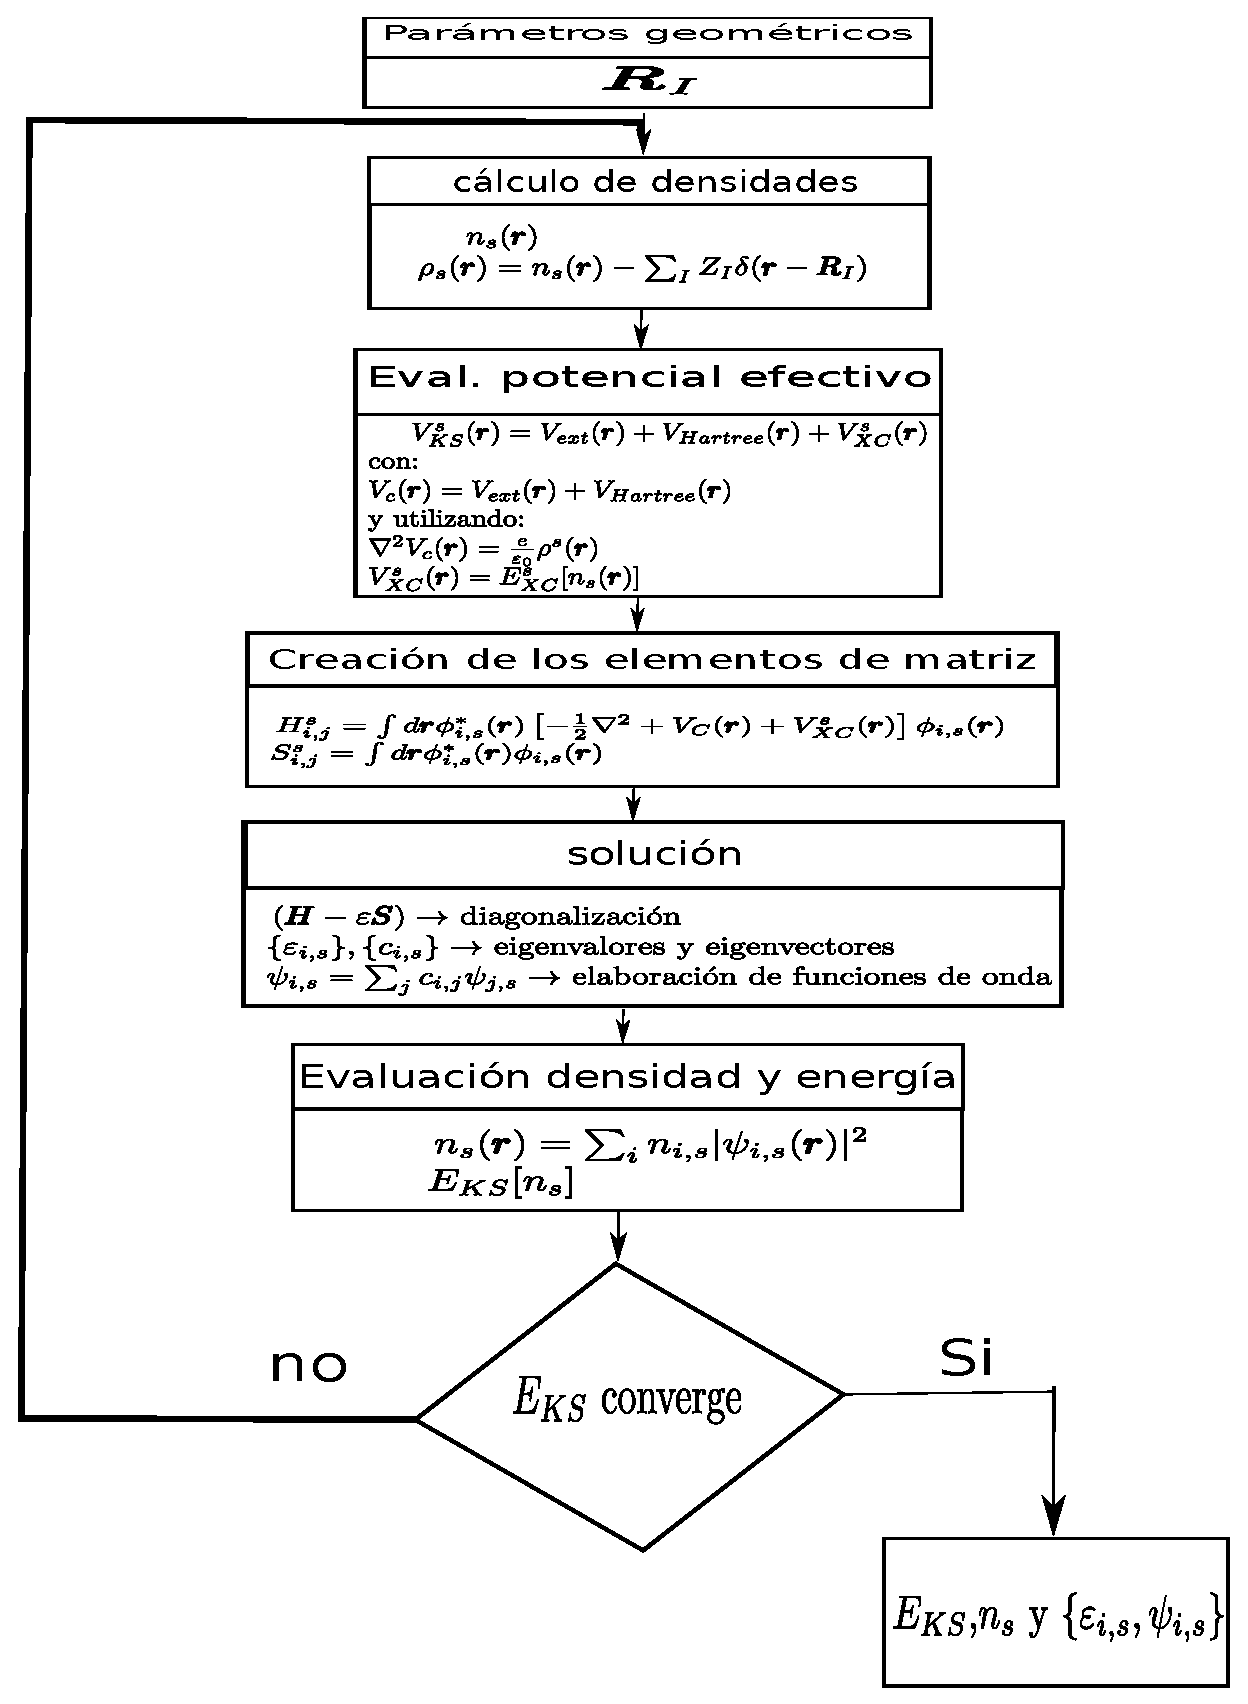
\epsfig{file=figuras/diagramaAuto.eps, width=15.0cm,height=19cm}
   	\caption[Diagrama de evaluaci\'on auto consistente]{Ciclo para resolver de forma auto consistente las ecuaciones de Kohn-Sham.}
   	\label{fig:esq}
   \end{figure}
   \newline
   \par En el caso de los spines no colineales no es posible separar la funci\'on de onda $\phi_{\Lambda} (\pmb{r},s)\not = \psi_{i,s } (\pmb{r}_j) \alpha_i (s_j) $, en donde $\Lambda$ representa los n\'umeros cu\'anticos  del orbital. Tambi\'en es necesario agregar un nuevo t\'ermino a la ecuaci\'on \ref{ec:ShKS} llamado campo magn\'etico de intercambio y correlaci\'on \cite{PhysRevB.37.10685}:
   \begin{equation*}
   B_{XCj} (\pmb{r}) = - \frac{\delta E_{XC} [n,\pmb{m}]}{\delta m_j (\pmb{r})} \label{ec:Bxc},
   \end{equation*}
   el cual representa un campo magn\'etico interno inducido por  los efectos de intercambio y correlaci\'on y en lugar de un sistema de dos ecuaciones  para el caso colineal, se tiene que resolver un sistema de cuatro ecuaciones \cite{MB-2015}:
   \begin{multline}
   \sum_{s}  \left[-\frac{1}{2} \nabla^2 + V_{ext} (\pmb{r})+ V_{Hartree} (\pmb{r}) + V_{XC} (\pmb{r}) \right] \delta_{s',s}  \phi_{\Lambda} (\pmb{r},s)\\ - \mu_{B} \sum_{s}  [\pmb{B}_{ext} (\pmb{r})+ \pmb{B}_{XC} (\pmb{r}) ] \cdot \pmb{\sigma_{s,s'}} \phi_{\Lambda} (\pmb{r},s) = \varepsilon_{\Lambda} \phi_{\Lambda} (\pmb{r},s) , \label{ec:KSnoColl}
   \end{multline}
   en donde $s$ toma los valores de $\uparrow, \downarrow$ y  las dos componentes del spinor correspondiente a cada orientaci\'on. As\'i mismo hay que considerar el acople spin \'orbita tal como se muestra en la secci\'on \ref{sec:Ho-Ko}.
   \subsection{Evaluaci\'on no auto consistente} \label{subsec:nscf}
   Cuando es necesario calcular estructuras de bandas o la densidad de estados, se utiliza una red mas densa en el espacio rec\'iproco (Sec. \ref{sec:solespacioK}). En este caso no es pr\'actico realizar el ciclo auto consiente y entonces lo que se hace es tomar la densidad de carga obtenida por la evaluaci\'on auto consistente con un n\'umero menor de puntos en el espacio rec\'iproco  y resolver la ecuaciones de Kohn-Sham (Ecs. \ref{ec:ShKS}-\ref{ec:potKS}), con el n\'umero de puntos en el espacio rec\'iproco deseado y obteniéndose así  una nueva densidad $n_0$,  dado que puede variar la magnitud de la densidad obtenida por este m\'etodo con respecto al que se obtiene con una evaluaci\'on auto consistente, se utiliza el  funcional de Harris  para evaluar la energ\'ia total del sistema debido a que es menos sensible a los cambios en $n_0$ que el potencial de Kohn-Sham. Este funcional est\'a dado por\cite{PhysRevB.31.1770}:
   \begin{equation}
   E_{Harris} [n_0] = \sum_{i} \varepsilon_i - \int d^3 r V_{ext} [n_0] n_0 (\pmb{r}) - \frac{1}{2} \int d^3 r V_{Hartree} [n_0] n_0 (\pmb{r}) + E_{XC} [n_0]. \label{ec:FuncHarris}
   \end{equation}
  
   \section{Funcional de intercambio y correlaci\'on ($E_{XC} $)}\label{sec2:xc}
   \subsection{Propiedades del funcional $E_{XC} $ exacto } \label{susec:exXC}
   El funcional de la energ\'ia de intercambio y correlaci\'on (Ec. \ref{ec:Exc2} )  se puede escribir como \cite{MB-2015}:
   \begin{equation}
   E_{XC}^s [n_s] = \int d \pmb{r} n_s (\pmb{r}) \epsilon_{XC} (\pmb{r}; [n_s]) \label{ec:enGenXCf},
   \end{equation} 
   donde $ \epsilon_{XC} (\pmb{r}; [n_s])$ es la energ\'ia de intercambio y correlaci\'on por part\'icula; en el caso de que los spines no est\'en orientados colinealmente se tiene que considerar la magnetizaci\'on y la polarizaci\'on.
   \newline
   \par Para analizar la contribuci\'on de $E_{XC} $ se utiliza el m\'etodo de conexi\'on adiab\'atica \cite{PhysRevA.29.1648}, en el que el cambio de la energ\'ia del sistema con respecto al par\'ametro $\lambda$ es igual al elemento de matriz de la derivada del Hamiltoniano con respecto al mismo par\'ametro. Entonces se puede calcular la energ\'ia entre dos estados $\lambda_1$ y $\lambda_2$ a través de una integral sobre una variaci\'on  del Hamiltoniano, que var\'ie de  $\lambda_1$ a $\lambda_2$. La denominaci\'on  de conexi\'on adiab\'atica se debe a que se asume que el Hamiltoniano que conecta los dos estados est\'a en el estado base para el valor de $\lambda$ y las expresiones generales son  dadas por \cite{Martin-2004, PhysRevA.29.1648}:
   \begin{equation}
   \frac{\partial E_0}{\partial \lambda} = \frac{\partial}{\partial \lambda} \left \langle \Psi_0^{\lambda} \left | \hat{H}_0 ^{\lambda} \right |  \Psi_0^{\lambda} \right \rangle = \left \langle \Psi_0^{\lambda} \left | \frac{\partial \hat{H}_0 ^{\lambda}}{\partial \lambda} \right |  \Psi_0^{\lambda} \right \rangle \label{ec:adAproxderivada}
   \end{equation}  
   o escrito en forma de integral:
   \begin{equation}
   \Delta E_0 = \int_{\lambda_1}^{\lambda_2} d \lambda~ \frac{\partial E_0}{\partial \lambda} = \int_{\lambda_1}^{\lambda_2} d \lambda \left \langle \Psi_0^{\lambda} \left | \frac{\partial \hat{H}_0 ^{\lambda}}{\partial \lambda}  \right |  \Psi_0^{\lambda} \right \rangle \label{ec:adAproxInt}.
   \end{equation}
   Se  escala el t\'ermino de la interacci\'on entre electrones $\lambda \hat{V}_{int}$ con el par\'ametro $\lambda (0 \le \lambda \le 1)$ entre un sistema sin interacci\'on ($\lambda=0$) y uno con interacci\'on ($\lambda=1$) y  se asume que $n(\pmb{r})= n^{\lambda} (\pmb{r})$, entonces es posible definir el siguiente Hamiltoniano \cite{Harris1974TheSE}: 
   \begin{equation}
   \hat{H}_{0}^{\lambda} = \hat{T}+ \hat{V}_{ext}^{\lambda}+ \lambda \hat{V}_{int} \label{ec:SH1Elec},
   \end{equation}
   en donde se reemplaza el potencial externo $\hat{V}_{ext} $ con $\hat{V}_{ext}^{\lambda} $ para garantizar que no cambie la densidad, utilizando las ecuaciones \ref{ec:adAproxderivada} y \ref{ec:adAproxInt} se puede escribir el funcional de la energ\'ia del estado base (Ec. \ref{ec:funcional} con $\pmb{B}_{ext}=0$) como  \cite{MB-2015}:
   \begin{subequations}
   	\begin{equation*}
   	E_0 = E_{V_{ext}} [n] = \langle \Psi_0^1 | \hat{H}_0 ^ 1 | \Psi_0^1 \rangle
   	\end{equation*}
   	\begin{equation*}
   	=\langle \Psi_0^0 | \hat{H}_0 ^ 0 | \Psi_0^0 \rangle + \int_{0}^{1} d \lambda \frac{\partial}{\partial \lambda } \left \langle \Psi_0^{\lambda} \left | \hat{H}_0 ^{\lambda} \right |  \Psi_0^{\lambda} \right \rangle
   	\end{equation*}
   	\begin{equation*}
   	=\langle \Psi_0^0 | \hat{H}_0 ^ 0 | \Psi_0^0 \rangle + \int d \pmb{r} [V_{ext}^1 (\pmb{r})-V_{ext}^0 (\pmb{r})] n (\pmb{r}) + \int_{0}^{1} d \lambda  \left \langle \Psi_0^{\lambda} \left | \hat{V}_{int} \right |  \Psi_0^{\lambda} \right \rangle
   	\end{equation*}
   \end{subequations}
   y asumiendo  que $V_{ext}^1 (\pmb{r}) \equiv V_{ext} (\pmb{r})$:
   \begin{equation*}
   E_0 = E_{V_{ext}} [n]= \langle \Psi_0^0 | \hat{T} | \Psi_0^0 \rangle + \int d \pmb{r} V_{ext} (\pmb{r}) n (\pmb{r}) + \int_{0}^{1} d \lambda  \left \langle \Psi_0^{\lambda} \left | \hat{V}_{int} \right |  \Psi_0^{\lambda} \right \rangle ;
   \end{equation*}
   dado que el primer t\'ermino corresponde a $T_{sp}$, se puede encontrar una nueva expresi\'on para $E_{XC}$ \cite{Martin-2004}: 
   \begin{equation}
   E_{XC} [n] = \int_{0}^{1} d \lambda  \left \langle \Psi_0^{\lambda} \left | \hat{V}_{int} \right |  \Psi_0^{\lambda} \right \rangle-E_{Hartree} = \frac{1}{2} \int d \pmb{r} n(\pmb{r})\int d \pmb{r'}  \frac{\widetilde{n }_{xc}(\pmb{r},\pmb{r'})}{|\pmb{r}-\pmb{r'}|} \label{ec:Exc3},
   \end{equation}
   en donde $\widetilde{n }_{xc} (\pmb{r},\pmb{r'})$ se define como \cite{Martin-2004}:
   \begin{equation}
   \widetilde{n }_{xc} (\pmb{r},\pmb{r'}) = \int_{0}^{1} d \lambda n_{xc}^{\lambda} (\pmb{r},\pmb{r'}) \label{ec:avHole}.
   \end{equation}
   Las ecuaciones \ref{ec:enGenXCf} y \ref{ec:Exc3} se utilizan para  escribir la energ\'ia de intercambio y correlaci\'on por part\'icula $\epsilon_{XC} $ como:
   \begin{equation}
   \epsilon_{XC} (\pmb{r}; [n])= \frac{1}{2} \int d \pmb{r'}  \frac{\widetilde{n }_{xc}(\pmb{r},\pmb{r'})}{|\pmb{r}-\pmb{r'}|} \label{ec:densEXC}.
   \end{equation}
     Se puede expresar el potencial de intercambio y correlaci\'on en funci\'on de la energ\'ia de intercambio y correlaci\'on por part\'icula \cite{PhysRevA.29.1648} como:
   \begin{equation}
   V_{XC} (\pmb{r}) = \epsilon_{XC} (\pmb{r}; [n]) + n(\pmb{r}) \frac{\delta \epsilon_{XC} (\pmb{r}; [n])}{\delta n(\pmb{r}) } \label{ec:potXC}.
   \end{equation}  
   La generalizaci\'on para el caso de spines colineales es \cite{Martin-2004}:
   \begin{equation}
   V_{XC}^s (\pmb{r}) = \epsilon_{XC} (\pmb{r}; [n]) + n(\pmb{r}) \frac{\delta \epsilon_{XC} (\pmb{r}; [n])}{\delta n_s(\pmb{r}) } , \label{ec:potXCspin}
   \end{equation}
   en donde se toma en cuenta que $\epsilon_{XC} \equiv \epsilon_{XC} \left(\pmb{r}; \left[ n_{\uparrow}, n_{\downarrow} \right]\right) $ es un funcional de las dos densidades de spines.
\newline
   \par Una de las primeras aproximaciones que se realizaron a la energ\'ia de intercambio y correlaci\'on fue la aproximaci\'on local de la densidad (LDA, por sus siglas en ingl\'es) \cite{PhysRev.140.A1133}, la cual presenta errores tales como la sobre estimaci\'on de  las energ\'ias de cohesi\'on de casi todos ls s\'olidos; adem\'as de la subestimaci\'on de los par\'ametros de red en varios casos, as\'i como  los errores al momento de describir sistemas altamente correlacionados y en especial presenta problemas con \'atomos de metales de transici\'on \cite{MB-2015}. Una forma de corregir estos inconvenientes es incluir correcciones de gradientes de la densidad para que la energ\'ia de intercambio y correlaci\'on pueda ser escrita en funci\'on de una densidad de energ\'ia de intercambio y correlaci\'on $g_{r} [n]$ \cite{MB-2015}:
   \begin{equation}
   E_{XC} [n]= \int d^3~ r g_{r} [n]
   \end{equation}
   y esta densidad se puede expandir en series \cite{PhysRevLett.22.807}:
$
   g_{r} [n] = g_0 (n(\pmb{r}))+ g_1 (n(\pmb{r})) [\nabla n(\pmb{r})]+ \ldots~
 .$
   Dicha  teor\'ia fue propuesta por Kohn y Sham\cite{PhysRev.140.A1133} aunque \'esta no soluciona los principales problemas de LDA. Por tal motivo se implement\'o la aproximaci\'on de gradientes generalizados (GGA, por sus siglas en ingl\'es) cuya expresi\'on para la energ\'ia de intercambio y correlaci\'on est\'a dada por \cite{Perdew1996ComparisonSF}:
   \begin{multline}
      E_{XC}^{GGA} [n_{\uparrow} (\pmb{r}), n_{\downarrow}(\pmb{r})] = \int d^3 r ~ n(\pmb{r}) \epsilon_{XC} \left(n_{\uparrow} (\pmb{r}), n_{\downarrow}(\pmb{r}), \left|\nabla n_{\uparrow} (\pmb{r}) \right|^2, \left|\nabla n_{\downarrow} (\pmb{r}) \right|^2 \right)  \\
      = \int d^3 r ~ n(\pmb{r}) \epsilon_{X}^{hom} (n) F_{XC} \left(n_{\uparrow} (\pmb{r}), n_{\downarrow}(\pmb{r}), \left|\nabla n_{\uparrow} (\pmb{r}) \right|^2, \left|\nabla n_{\downarrow} (\pmb{r}) \right|^2 \right), \label{ec:funcXCGGA}
   \end{multline}
   en donde $ \epsilon_{X}^{hom} (n) = -3k_F / 4\pi $ es la energ\'ia de intercambio por part\'icula  de un gas de electrones homog\'eneo no polarizado y  $k_F = (3 \pi^2 n)^{1/3}$ es el vector de onda de Fermi y $F_{XC}$ es una funci\'on adimensional de las densidades y sus gradientes \cite{Martin-2004}. Dicha funcional \ref{ec:funcXCGGA} se denota un funcional XC semilocal. Es importante tomar en cuenta que es posible separar la parte correspondiente a la correlaci\'on de la de intercambio de la siguiente manera: $ \epsilon_{XC} (\pmb{r}; [n] )= \epsilon_{X} (\pmb{r}; [n] )+ \epsilon_{C} (\pmb{r}; [n] ) $ y por lo tanto tambi\'en es v\'alido realizar la siguiente divisi\'on $ F_{XC} = F_{X}+ F_{C} $ \cite{MB-2015}.
   \newline
   \par Una de las aproximaciones mas utilizadas es la desarrollada por Perdew, Burke y Enzerhof (PBE) en donde la parte correspondiente a el intercambio puede ser escrita de la siguiente forma \cite{PhysRevLett.77.3865, mo_2004}:
   \begin{equation}
   E_X [n_{\uparrow}, n_{\downarrow}]= \frac{1}{2} \left[E_{X} [2 n_{\uparrow}] + E_{X} [2 n_{\downarrow}]   \right]. \label{ec:divEx}
   \end{equation}
   Adem\'as se puede definir el gradiente de densidad reducida como:
   \begin{equation}
   s(\pmb{r})= \frac{|\nabla n (\pmb{r})|}{2 k_F n (\pmb{r}) }. \label{ec:S}
   \end{equation}
   Por tanto  $F_X (s)$ queda dada por:
   \begin{equation}
   F_{X}^{PBE} = 1+\kappa -\frac{\kappa}{1+\mu s^2 /\kappa}, \label{ec:F_X-PBE}
   \end{equation}
   donde $\mu = 0.21951 $ y $\kappa= 0.804 $. La energ\'ia de correlaci\'on est\'a dada por \cite{mo_2004}:
   \begin{equation}
   E_{C} ^{PBE} = \int d^3 r n \left\{\epsilon_{C}(r_s,\zeta)+ H^{PBE} (r_s,\zeta,t), \right\}\label{ec:funcCorr},
   \end{equation}
   donde $r_s = (3/4 \pi n)^{1/3}, ~ \zeta =(n_{\uparrow}-n_{\downarrow})/n,~ t=|\nabla n|/2 k_s \phi n, ~\phi= \frac{1}{2} [(1+\zeta)^{2/3}+(1-\zeta)^{2/3}],~ k_s = (4 k_F/\pi)^{1/2}$,
   \begin{equation}
   H^{PBE} = \gamma \phi^3 \ln \left\{1+ \frac{\beta}{\gamma} t^2 \left[\frac{1+At^2}{1+At^2+A^2 t^4}\right]\right\}, \label{ec:PBEH}
   \end{equation}
   \begin{equation}
   A=\frac{\beta}{\gamma} [exp\{-\epsilon_{C}^{hom}/\gamma \phi^3 \}-1]^{-1} \label{ec:A}
   \end{equation}
   y $\gamma=0.031091, ~\beta=0.066725$. Los gradientes reducidos $s$ y $t$ miden qu\'e tan r\'apido $n(\pmb{r})$ var\'ia en las escalas de la longitud de onda de Fermi $2\pi/k_F$ y el apantallamiento de Thomas-Fermi $1/k_s$ respectivamente. Esta clase de funcionales mejoran los resultados obtenidos con LSDA \cite{MB-2015}.
   \newline
   \par Para calcular el potencial de intercambio y correlaci\'on encontrando el cambio $\delta E_{XC} [n]$ con respecto a un cambio  $\delta n$ y $\nabla \delta n$, se usa la siguiente expresi\'on \cite{Martin-2004}:
   \begin{equation}
   \delta E_{XC} [n] = \sum_{s} \int d \pmb{r} \left[\epsilon_{XC} + n \frac{\partial \epsilon_{XC}}{\partial n_s} + n \frac{\partial \epsilon_{XC}}{\partial \nabla n_s} \right]_{\pmb{r},s} \delta n_s(\pmb{r}), \label{ec:ecpotVXC_1}
   \end{equation}
   en donde el termino dentro de los par\'entesis cuadrados no se puede considerar como un potencial local debido al \'ultimo t\'ermino. Existen tres aproximaciones para manejar este t\'ermino, la primera es encontrar el potencial local $V_{XC}^s (\pmb{r})$ por interacci\'on  del \'ultimo  t\'ermino \cite{Martin-2004}:
   \begin{equation}
   V_{XC}^s (\pmb{r}) = \left[\epsilon_{XC}+\frac{\partial \epsilon_{XC}}{\partial n_s}- \nabla \left(n \frac{\partial \epsilon_{XC}}{\partial \nabla n_s}\right) \right] \label{ec:potXC_2},
   \end{equation}
   el cual es el mas usado pero tiene como desventaja que requiere derivadas de mayor orden para la densidad, lo cual crea dificultades num\'ericas.
   \newline
   \par La segunda aproximaci\'on es usar un operador de la forma dada por ecuaci\'on \ref{ec:potXC} directamente para modificar las ecuaciones de Kohn-Sham. Usando el hecho de que la densidad se puede escribir en t\'erminos de las funciones de onda $\psi_i$, el elemento de matriz quedar\'ia como \cite{PhysRevLett.76.660}:
   \begin{equation}
   \langle \psi_i |\hat{V}_{XC}| \psi_i \rangle = \int \left[\tilde{V}_{XC} \psi_i ^* \psi_i + \psi_i ^* \pmb{V}_{XC} \cdot \nabla \psi_i + (\pmb{V}_{XC} \cdot \nabla \psi_i^*) \psi_i \right], \label{ec:potXC_3}
   \end{equation}
   donde $\tilde{V}_{XC} = \epsilon_{XC} + n (\partial \epsilon_{XC}/ \partial n)$ y $\pmb{V}_{XC} = n (\partial \epsilon_{XC} / \partial \nabla n) $. Esta forma es mas estable en t\'erminos num\'ericos pero requiere la inclusi\'on de operaciones vectoriales en la ecuaci\'on de Kohn-Sham lo cual incrementa  el respectivo trabajo computacional \cite{Martin-2004}.
   \newline
   \par Finalmente, la tercera aproximaci\'on fue propuesta por White y Bird \cite{PhysRevB.50.4954} que consiste en tratar $E_{XC}$ como una funci\'on de la densidad, donde los t\'erminos de  los gradientes son definidos por un operacional en funci\'on de la densidad. Entonces la ecuaci\'on \ref{ec:potXC} puede ser escrita usando la regla de la cadena:
   \begin{multline}
   \delta E_{XC} [n] = \sum_{s} \int d \pmb{r} \left[\epsilon_{XC} + n \frac{\partial \epsilon_{XC}}{\partial n_s} \right] \delta n_s (\pmb{r}) \\
   + \sum_{s}  \int\int d  \pmb{r} d \pmb{r'} n(\pmb{r}) \left[\frac{\partial \epsilon_{XC}}{\partial \nabla n_s} \right] ~ \frac{\delta \nabla n(\pmb{r'})}{\delta n(\pmb{r})} \delta n_s (\pmb{r}), \label{ec:potXC_4}
   \end{multline}
   donde $ (\delta n(\pmb{r'})/\delta n(\pmb{r}))$ denota una derivada funcional. Tambi\'en se puede notar que la densidad est\'a dada por puntos discretos en una red $n(\pmb{r}_m)$ en donde el gradiente $\nabla n(\pmb{r}_m) $ puede ser  determinado mediante \cite{PhysRevB.50.4954}:
   \begin{equation}
   	\nabla n(\pmb{r}_m)= \sum_{m} \pmb{C}_{m-m'} n(\pmb{r}_m) \label{ec:gradDisc}
   \end{equation}  
   y la derivada funcional tiene la siguiente forma:
   \begin{equation}
   \frac{\delta \nabla n(\pmb{r}_m)}{\delta n(\pmb{r}_m')} \rightarrow \frac{\partial \nabla n(\pmb{r}_m)}{\partial n(\pmb{r}_m')} = \pmb{C}_{m-m'}, \label{ec:gradCmm}
   \end{equation}
   en donde $\pmb{C}_{m} = \{ C_m ^x , C_m ^y , C_m ^z  \}$  es un vector en las coordenadas espaciales. Si se utilizan los coeficientes $\pmb{C}_m$ que son diferentes de cero en un rango finito y variando $n_s (\pmb{r}_m)$ en la expresi\'on para $E_{XC}$ y utilizando la regla de la cadena, se obtiene que \cite{PhysRevB.50.4954}:
   \begin{equation}
   V_{XC}^s (\pmb{r}_m) = \left[\epsilon_{XC}+n \frac{\partial \epsilon_{XC}}{\partial n}\right]_{\pmb{r}_{m, s}} + \sum_{s'} \left[ n \frac{\partial \epsilon_{XC}}{\partial |\nabla n|} ~\frac{\nabla n}{\partial |\nabla n|}\right] _{\pmb{r}_{m', s}} \pmb{C}_{m'-m} \label{ec:potVxc}.
   \end{equation}
   Esta expresi\'on para el potencial reduce los problemas num\'ericos asociados con la expresi\'on \ref{ec:potXC_2} sin utilizar operadores vectoriales como en la ecuaci\'on \ref{ec:potXC_3}. Adem\'as que se puede notar que $V_{XC}^s (\pmb{r}_m)$ es una funci\'on no local de $n_s (\pmb{r}_m)$.
   \section{Formalismo  en el espacio K}\label{sec:solespacioK}
   Debido a que generalmente los problemas que se tratan son s\'olidos cristalinos, entonces es conveniente  utilizar como funciones base a ondas planas para la expansi\'on de las eigenfunciones para las ecuaciones de Kohn-Sham (ec. \ref{ec:HamiltonianoKS}). Para un sistema  translacionalmente invariante las ondas planas est\'an dadas por \cite{MB-2015}
   \begin{equation}
   \phi_{\pmb{k},\pmb{G}} (\pmb{r})= \frac{1}{\sqrt{\Omega}} e^{i (\pmb{k}+\pmb{G})\cdot \pmb{r}} \label{ec:ondaplana},
   \end{equation}
   en donde $\Omega$ es el volumen del sistema y $\pmb{k} $ est\'a en la primera zona de Brillouin y $\pmb{G}$ est\'a en la red rec\'iproca. Adem\'as \'este conjunto de ondas planas es ortonormal \cite{MB-2015}:
   \begin{equation}
   \int d \pmb{r} \phi_{\pmb{k},\pmb{G}}^* (\pmb{r}) \phi_{\pmb{k},\pmb{G}} (\pmb{r}) = \delta_{\pmb{k}, \pmb{k'}} \delta_{\pmb{G}, \pmb{G'}} \label{ec:PWorto}
   \end{equation} 
   y completo
   \begin{equation}
   \sum_{\pmb{k}} \sum_{\pmb{G}}  \phi_{\pmb{k},\pmb{G}} (\pmb{r}) \phi_{\pmb{k},\pmb{G}}^* (\pmb{r'}) = \delta (\pmb{r}- \pmb{r'}). \label{ec:PWComp}
   \end{equation}
   Para un sistema translacionalmente invariante cada eigenfunci\'on de Kohn-Sham $\psi_{v,\pmb{k},s }$ que cumple con el teorema de Bloch, se puede expandir como \cite{Martin-2004}:
   \begin{equation}
   \psi_{v,\pmb{k},s } (\pmb{r}) = \sum_{\pmb{G}} c_{v,\pmb{k},s } \phi_{\pmb{k},\pmb{G}} (\pmb{r}), \label{ec:basePW}
   \end{equation}
   en donde $v$ es el \'indice de la banda con  spin $s$. La densidad cumple con $n_s (\pmb{r}) = n_(s) (\pmb{r}+\pmb{R})$ y toma la siguiente forma \cite{MB-2015}:
   \begin{eqnarray}
   n_s(\pmb{r}) &=& \sum_{\pmb{G}} e^{-i \pmb{G} \pmb{r}} \tilde{n}_s (\pmb{G})  \label{ec:desnsiadK},\\
   \tilde{n}_s (\pmb{G}) &=& \frac{1}{\Omega} \sum_{v,\pmb{k}} n_{v,\pmb{k},s} \sum_{\pmb{G'}} c_{v,\pmb{k},s}^* (\pmb{G'}+\pmb{G}) c_{v,\pmb{k},s} (\pmb{G'}). \nonumber
   \end{eqnarray}
   Por lo tanto las ecuaciones de Kohn-Sham \ref{ec:ShKS} toman la siguiente forma \cite{doi:10.1080/00018738700101042}:
   \begin{equation}
   \sum_{\pmb{G'}} \left\{ \left[\frac{1}{2} (\pmb{k}+ \pmb{G})^2 - \varepsilon_{v,s} (\pmb{k}) \right] \delta_{\pmb{G},\pmb{G'}} + V_{KS} ^ s (\pmb{G}-\pmb{G'}) \right\} c_{v,\pmb{k},s} (\pmb{G'}) =0 \label{ec:HKSRes}
   \end{equation} 
   con la energ\'ia de banda $\varepsilon_{v,s} (\pmb{k})$. Se consideran los coeficientes de Fourier $V_{KS} ^ s (\pmb{G}-\pmb{G'})$ de un potencial local.
   \newline
   \par El uso de ondas planas (ec. \ref{ec:basePW}) se puede interpretar como el uso de una red en el espacio rec\'iproco como se ilustra en la figura \ref{fig:a-espacioK}. Para grandes vol\'umenes $\Omega$ se necesita un gran n\'umero de ondas planas pero debido  a que se est\'a utilizando sistemas peri\'odicos, se tiene que la cantidad de puntos $\pmb{k}$ en la primera zona de Brillouin est\'a dado por $\sum_{\pmb{k}} = \frac{\Omega}{(2 \pi )^3} \Omega_{BZ}$ \cite{MB-2015},  en donde el volumen de la zona de Brillouin est\'a dado por $\Omega_{BZ} =\frac{(2 \pi )^3}{\Omega_0} $ y $\Omega_0$ es el volumen de la celda unitaria.
   
   \begin{figure}[!htb]
   	\centering
   	\subfigure[]
   	{
   		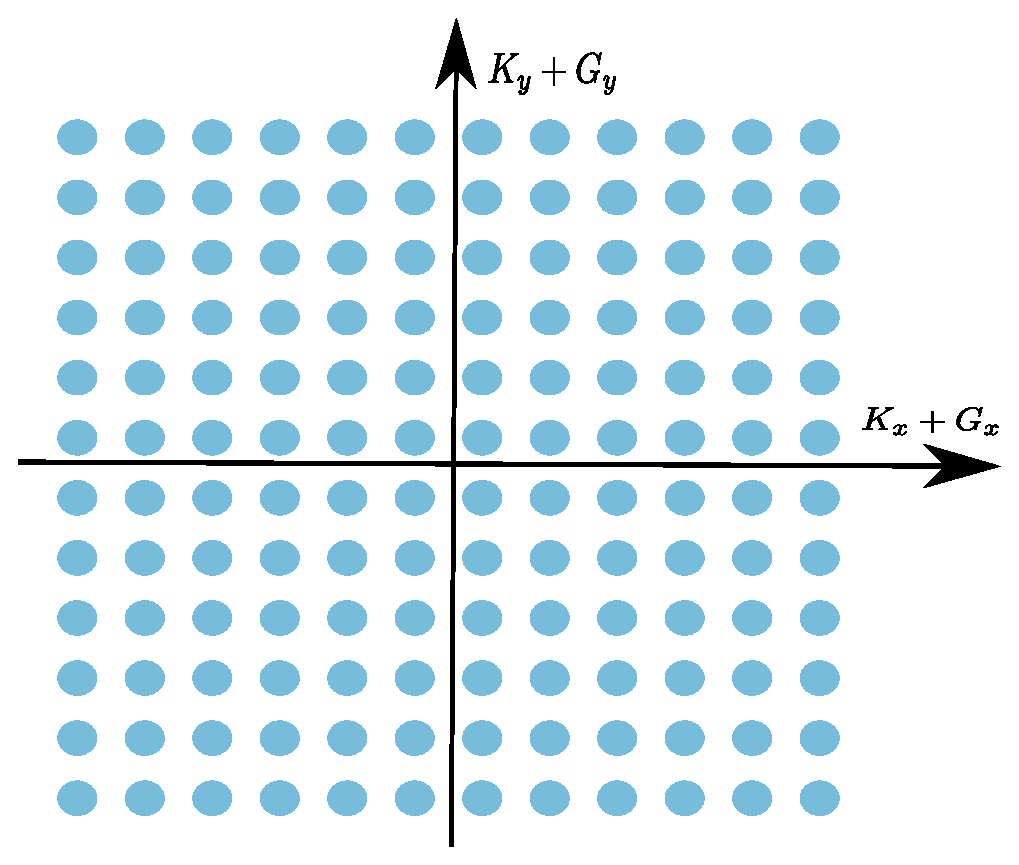
\epsfig{file=figuras/epacioKa.eps, width=5.0cm,height=5.0cm}
   		\label{fig:a-espacioK}
   	}
   \subfigure[]{
   	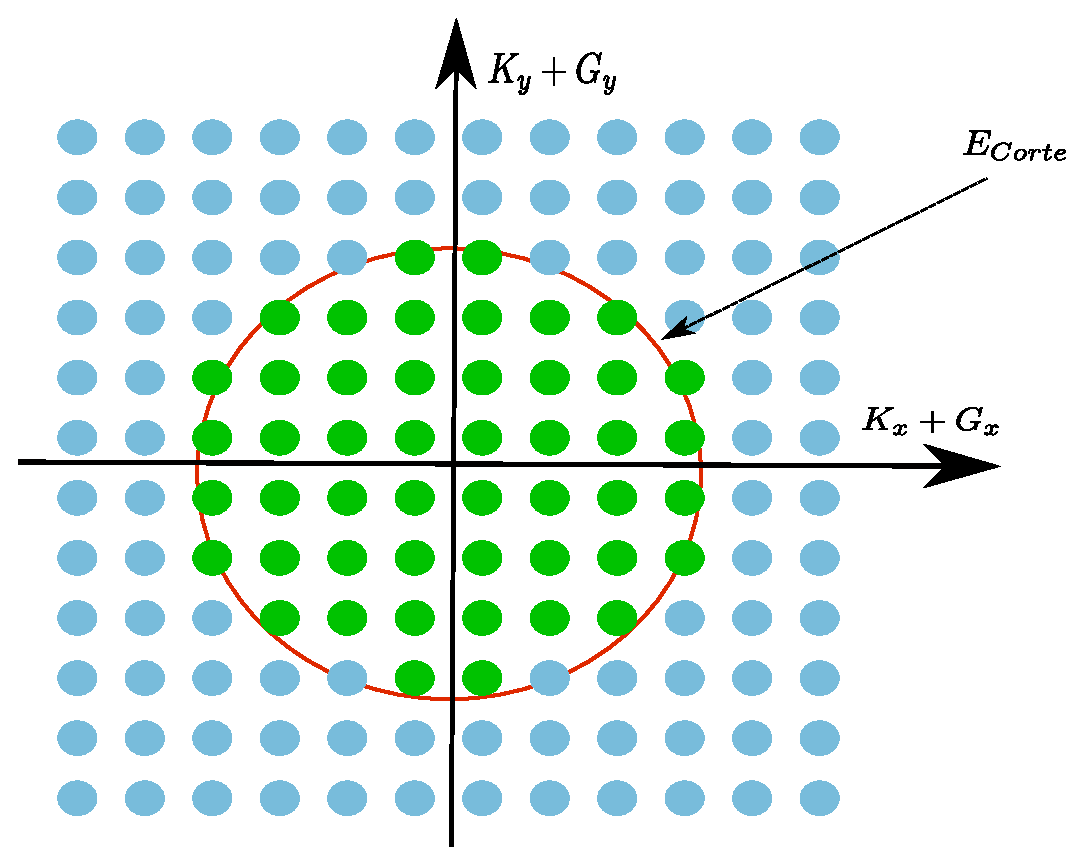
\epsfig{file=figuras/epacioKb.eps, width=5.0cm,height=5.0cm}
   	\label{fig:b-espacioK}
   }
   \caption[Mapeo espacio rec\'iproco]{en la figura \ref{fig:a-espacioK} se muestra el mapeo en el espacio rec\'iproco usando ondas planas. En la figura \ref{fig:b-espacioK} e muestra c\'omo  se trunca el espacio rec\'iproco por medio de la energ\'ia de corte $E_{corte}$\cite{MB-2015}.}
   \label{fig:espacioK}
   \end{figure}
   En la pr\'actica el n\'umero de ondas planas es limitado a una energ\'ia de corte $E_{corte}$ relacionada con la energ\'ia cin\'etica \cite{MB-2015}:
   \begin{equation}
   \int d \pmb{r}  \phi_{\pmb{k},\pmb{G}}^* (\pmb{r}) \left\{-\frac{1}{2} \nabla^2 \right\} \phi_{\pmb{k},\pmb{G}} (\pmb{r}) = \frac{1}{2} (\pmb{k}+ \pmb{G})^2 \le E_{corte}. \label{ec:Ecut}
   \end{equation}
   Esta energ\'ia determina el n\'umero de ondas planas que se usan en el c\'alculo y resultan al truncar el espacio rec\'iproco como se muestra en la figura \ref{fig:b-espacioK}, cuyo volumen es $\frac{4 \pi }{3} (2 E_{corte})^{3/2}$. Entonces el n\'umero de ondas planas por \'atomo $N_{PW}$ es \cite{PhysRevB.61.4576}:
   \begin{equation}
   N_{PW}\cdot N_{atomo} \approx \frac{4 \pi }{3} \frac{(2E_{corte})^{3/2}}{\Omega_{BZ}}. \label{ec:NumAtomoPW}
   \end{equation}
   Para muchos casos s\'olo se necesita una cantidad muy peque\~na de ondas planas tales como los \'atomos cuyos electrones de valencia pertenecen a los orbitales s y p si su comportamiento no se ve influido por los n\'ucleos. En el caso de que se tengan orbitales d se necesitar\'a una cantidad mayor de ondas planas debido a que estos estados est\'an mas localizados y por lo tanto se tienen que aumentar la energ\'ia de corte.
   \newline
   \par  La densidad y la energ\'ia total implican sumas en $\pmb{k}$ (o integrales sobre la primera zona de Brillouin ) y  se utilizan un n\'umero finito de  puntos en el espacio reciproco  resultando en un muestreo en la zona de Brillouin. El n\'umero de puntos depende de la dispersi\'on de las bandas ocupadas, donde t\'ipicamente se necesitan mas puntos $\pmb{k}$ para metales. anteriormente se tomaba en  cuenta  la simetr\'ia del sistema para obtener los puntos especiales $\pmb{k}^*$ en la zona irreducible de Brillouin; tales puntos eran suficientes para realizar estas sumas \cite{MB-2015}. Posteriormente se desarroll\'o   un m\'etodo para obtener estos puntos desarrollado por Monkhorst y Pack que realiza un muestreo con puntos $\pmb{k}$ equidistantes con pesos id\'enticos \cite{PhysRevB.13.5188}:
   \begin{equation}
   \pmb{k}_{n_1, n_2, n_3} = \sum_{i}^{3} \frac{2 n_i -N_i-1}{2N_i} \pmb{G}_i \label{ec:sampleMP}
   \end{equation}
   en donde $\pmb{G}_i $ son los vectores base del espacio rec\'iproco, $N_i$ es el n\'umero total de puntos en la direcci\'on $i$ y $n_i$ es el n]'umero de puntos \pmb{k} entre dos puntos en el espacio rec\'iproco conectados a trav\'es de  $\pmb{G}_i $.
    
   \section{C\'alculo de la Fuerza} \label{sec:Fuerza}
   \subsection{El teorema de Hellman-Feynman} \label{subsec:HellFey}
   Este teorema es de gran importancia en la f\'isica y el cual fue formulado Hellmann en 1937 \cite{Hellman-1937} y Feynman en 1939 \cite{PhysRev.56.340}, que consiste en obtener una expresi\'on  para la fuerza  que se ejerce en un n\'ucleo  y est\'a dado estrictamente en t\'erminos de la densidad electr\'onica independiente de la energ\'ia cin\'etica y de intercambio y correlaci\'on. Dicho  teorema tambi\'en es llamado  "Teorema de Fuerza" \cite{Martin-2004}. La fuerza puede ser escrita de la siguiente forma
   \begin{equation}
   \pmb{F}_I = - \frac{\partial E}{\partial \pmb{R}_I}. \label{ec:Fuerza}
   \end{equation} 
   Utilizando la expresi\'on general de la energ\'ia se obtiene la siguiente expresi\'on \cite{Martin-2004}
   \begin{equation}
   -\frac{\partial E}{\partial \pmb{R}_I} = - \left\langle \Psi \left| \frac{\partial \hat{H}}{\partial \pmb{R}_I} \right| \Psi \right\rangle- \left\langle \frac{\partial \Psi}{\partial \pmb{R}_I} \left| \hat{H} \right| \Psi \right\rangle - \left\langle \Psi \left| \hat{H} \right|  \frac{\partial \Psi}{\partial \pmb{R}_I} \right\rangle - \frac{\partial E_{II}}{\partial \pmb{R}_I}. \label{ec:expansionF}
   \end{equation}
   Utilizando el hecho de que se est\'a en el estado base se conoce que este es un extremo y por lo tanto los dos t\'erminos de en medio de la ecuaci\'on \ref{ec:expansionF} son cero. Por lo tanto la expresi\'on para la fuerza (omitiendo el spin) queda como \cite{MB-2015}:
   \begin{equation}
   \pmb{F}_I = -\frac{\partial E}{\partial \pmb{R}_I} = - \int d^3 r ~n(\pmb{r}) \frac{\partial V_{ext} (\pmb{r})}{\partial \pmb{R}_I}- \frac{\partial E_{II}}{\partial \pmb{R}_{II}}. \label{ec:FHFuerza} 
   \end{equation} 
   En el caso de que no se tenga un potencial local. no es posible expresar la fuerza en t\'erminos de la densidad electr\'onica pero a\'un es v\'alida la expresi\'on descrita anteriormente \cite{Martin-2004}
   \begin{equation}
   -\frac{\partial E}{\partial \pmb{R}_I} = - \left\langle \Psi \left| \frac{\partial \hat{H}}{\partial \pmb{R}_I} \right| \Psi \right\rangle - \frac{\partial E_{II}}{\partial \pmb{R}_I}. \label{ec:HFT}
   \end{equation}
   \subsection{C\'alculo auto consistente de fuerzas} \label{subsec:SConsFuerza}
   Es necesario redefinir la energ\'ia total $E_{tot} (\{\pmb{R}_I\})$ de un sistema con diferentes especies de n\'ucleos A,B, ..., los cuales est\'an fijos en las posiciones $\{\pmb{R}_I\} $ y en donde los electrones se mueven en un campo generado por los n\'ucleos $V_{ext} (\pmb{r})$. Las dos contribuciones mas importantes son la energ\'ia de los electrones en el estado base para cierta configuraci\'on $\{\pmb{R}_I\}$ de los n\'ucleos, la cual est\'a descrita por la energ\'ia de Kohn-Sham (ec. \ref{ec:funcHK} )  (omitiendo la constante de interacci\'on de los n\'ucleos y el spin) 
   \begin{multline}
   E_{KS} [n] = E_{V_{ext}} [n] = E_{KS} ([n],\{\pmb{R}_I\}) \\
   = T_{sp} [n] + \int d \pmb{r} V_{ext} n(\pmb{r}) + E_{Hartree} [n] + E_{XC} [n] \label{ec:KS_Fuerza}
   \end{multline}
   y la energ\'ia de la repulsi\'on de Coulomb  entre n\'ucleos ($E_{I I}$) (Sec. \ref{sec:introdft}, el \'ultimo t\'ermino es la ecuaci\'on \ref{ec:sh} ) se puede expresar como
   \begin{equation}
   	E_{II} = E_{nn} (\{\pmb{R}_I\}) = \frac{1}{2} \sum_{\substack{I,I' = 1 \\ (I \not = I')}}^ {N_n} Z_I Z_{I'} v(\pmb{R}_I - \pmb{R}_{I'}), \label{ec:IntII}
   \end{equation}
   en donde $ v(\pmb{R}_I - \pmb{R}_{I'})$ representa una interacci\'on de Coulomb. La energ\'ia total se puede representar como
   \begin{equation}
   E_{tot} (\{\pmb{R}_I\}) = E_{nn} (\{\pmb{R}_I\}) + E_{KS} ([n], \{\pmb{R}_I\}), \label{ec:EnTot2} 
   \end{equation}
   en donde  solo el potencial $V_{ext} (\pmb{r})$ depende expl\'icitamente de las coordenadas del n\'ucleo; as\'i mismo tampoco se consideran las vibraciones de red.
   \newline
   Para encontrar las posiciones $ \{\pmb{R}_I \}$ es necesario calcular la energ\'ia del estado base para la cierta configuraci\'on de $ \{\pmb{R}_I \}$ y para encontrar el m\'inimo global  de la energ\'ia total. Lejos del m\'inimo de la energ\'ia $E_{tot} (\{\pmb{R}_I\})$ existe una fuerza descrita por el teorema de Hellman-Feynman; en este caso se hace el cambio $\frac{\partial}{\partial \pmb{R}_I}  \rightarrow \nabla_{\pmb{R}_I}$ \cite{MB-2015}
   \begin{equation}
   \pmb{F}_I = - \nabla_{\pmb{R}_I} E_{tot} (\{\pmb{R}_I\}). \label{ec:Fuerza_Et}
   \end{equation}
   Para una dada composici\'on $N_A,N_B, ...$ y con cierta configuraci\'on $\{\pmb{R}_I\}$ la magnitud y la direcci\'on de una fuerza at\'omica provee informaci\'on acerca de que tan lejos est\'a cierto \'atomo de su posici\'on estable o metaestable, de tal forma que la geometr\'ia de equilibrio se determina cuando estas fuerzas netas son cero:
   \begin{equation}
   \pmb{F}_I |_{\{\pmb{R}_I\}= \{\pmb{R}_I^0\}} = 0 , ~~~~para~ todo~ I .\label{ec:fuerzaEq}
   \end{equation}
   La estructura \'optima $\{\pmb{R}_I^0\}$ de un s\'olido corresponde a un m\'inimo en la energ\'ia (ec. \ref{ec:EnTot2}). Este m\'inimo no es necesariamente el global y para encontrarlo se tienen que realizar m\'ultiples configuraciones y comparar la energ\'ia total. Usualmente se parte de una geometr\'ia inicial y se utiliza un segundo ciclo auto consistente para encontrar la geometr\'ia de equilibrio $\{\pmb{R}_I\}$. Este ciclo se muestra en la figura \ref{fig:esqFuerza}, el cual encapsula el ciclo auto consistente interno del c\'alculo de la energ\'ia, (fig. \ref{fig:esq}) \cite{MB-2015}.
   \begin{figure}[!hbt]
   	\centering
   	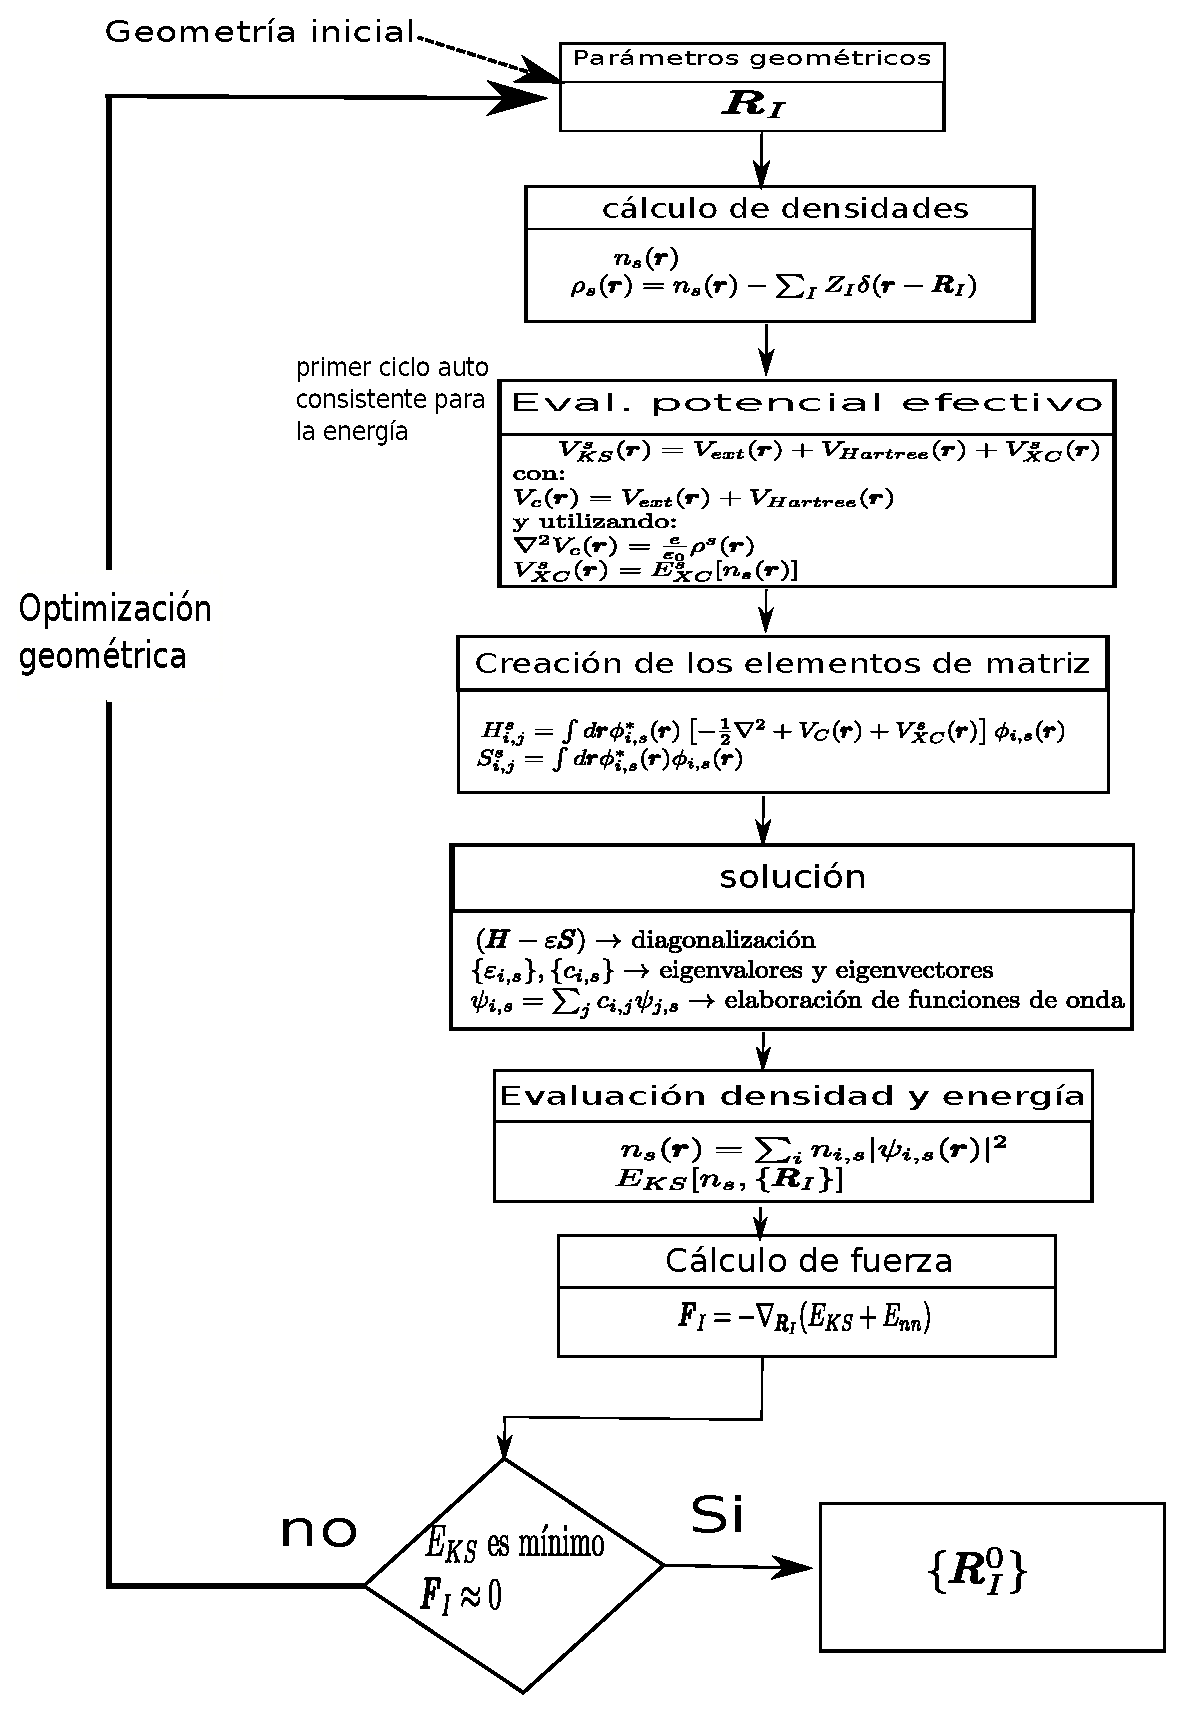
\epsfig{file=figuras/diagramaAuto2.eps, width=12.0cm,height=18.0cm}
   	\caption[C\'alculo auto consistente de fuerzas. ]{ciclo auto consistente para encontrar la geometr\'ia de equilibrio a partir de una geometr\'ia inicial $\{\pmb{R}_I^i\} $.}
   	\label{fig:esqFuerza}
   \end{figure}
   \newline
   Calculando las fuerzas de Hellman-Feynman utilizando la energ\'ia total (ec. \ref{ec:EnTot2}) se pueden obtener dos componentes \cite{doi:10.1080/00018738700101042}
   \begin{equation}
   	\pmb{F}_I = \pmb{F}_I^n + \pmb{F}_I^{el}, \label{ec:FuerzaDesc}
   \end{equation}
   en donde  la contribuci\'on debida a la repulsi\'on entre n\'ucleos es
   \begin{equation}
   \pmb{F}_I^n = \sum_{\substack{I,I' = 1 \\ (I \not = I')}}^{N_n} v(\pmb{R}_I - \pmb{R}_{I'}) \frac{\pmb{R}_I - \pmb{R}_{I'}}{|\pmb{R}_I - \pmb{R}_{I'}|^2}, 
   \end{equation}
   la cual es provocada por la energ\'ia de interacci\'on entre n\'ucleos (ec. \ref{ec:IntII}). Estudiando la contribuci\'on electr\'onica  (ec. \ref{ec:KS_Fuerza})se puede observar que s\'olo el potencial externo $V-{ext} (\pmb{r})$ depende expl\'icitamente de las posiciones nucleares $\{\pmb{R}_I\}$ y  la densidad $n(\pmb{r})$ depende impl\'icitamente de estas posiciones y acorde con el teorema de Hellman-Feynman (ec. \ref{ec:HFT}),  el \'ultimo t\'ermino en la ecuaci\'on \ref{ec:FuerzaDesc} se puede separar en dos t\'erminos \cite{doi:10.1080/00018738700101042}:
   \begin{equation}
   \pmb{F}_I^{el} = \pmb{F}_I^{el (1)} + \pmb{F}_I^{el (2)} \label{ec:descFel},
   \end{equation} 
   con
   \begin{equation}
   \pmb{F}_I^{el (1)} = - \int d \pmb{r} ~n(\pmb{r}) \nabla_{\pmb{R}_I} V_{ext} (\pmb{r}) \label{ec:Fel_1}
   \end{equation}
   y
   \begin{equation}
   \pmb{F}_I^{el(2)} = - \int d \pmb{r} \frac{\delta E_{KS} [n]}{\delta n(\pmb{r})} \nabla_{\pmb{R}_I} n(\pmb{r}). \label{ec:Fel_2} 
   \end{equation}
   De acuerdo con el segundo teorema de Hohenberg-Kohn, la ecuaci\'on \ref{ec:Fel_1} se hace cero cuando se logra el estado base del sistema. En tratamientos num\'ericos se pueden considerar fuerzas que se rigen con la ecuaci\'on \ref{ec:Fel_2}, las cuales se deben a inexactitudes num\'ericas en e c\'alculo de la densidad electr\'onica en el proceso observado en la figura \ref{fig:esqFuerza}. Usando la representaci\'on de la densidad electr\'onica en t\'erminos de los orbitales de Kohn-Sham $n(\pmb{r}) = \sum_i n_i |\psi_i (\pmb{r})|^2 $, la fuerza se puede como \cite{MB-2015}:
   \begin{equation}
   \pmb{F}_I^{el(2)} = -2 Re \sum_i n_i \int d \pmb{r} [\nabla_{\pmb{R}_I} \psi_i^* (\pmb{r})] \left[-\frac{1}{2} \nabla^2 + V_{KS} (\pmb{r}) - \varepsilon_i \right] \psi_i (\pmb{r}) \label{ec:F2scf}
   \end{equation}
   o
   \begin{eqnarray}
   \pmb{F}_I^{el(2)} = &-& 2 Re \sum_i n_i \int d \pmb{r} [\nabla_{\pmb{R}_I} \psi_i^* (\pmb{r})] \left[-\frac{1}{2} \nabla^2 + \tilde{V}_{KS} (\pmb{r}) -\varepsilon_i \right] \psi_i (\pmb{r}) \nonumber\\ 
   &-& \int d\pmb{r} [V_{KS} (\pmb{r})-\tilde{V}_{KS} (\pmb{r})] \nabla_{\pmb{R}_I} n(\pmb{r}). \label{ec:F2scf_2} 
   \end{eqnarray}
    El primer t\'ermino de la ecuaci\'on \ref{ec:F2scf_2} es cero si los cambios de las funciones de onda mantienen la orto-normalidad cuando un \'atomo se desplaza. Esto debe de cumplirse siempre cuando se utilizan  ondas planas como funciones base. 
      
   \section{Pseudopotenciales}\label{sec:pseudo}
   \subsection{Introducci\'on a los pseudopotenciales} \label{subsec:introPseudo}
   Es importante puntualizar que el uso de ondas planas solamente es una soluci\'on exacta si el potencial no var\'ia en el espacio y en el caso de que esta variaci\'on sea peque\~na  se puede tratar como una perturbaci\'on. Por lo general  el potencial externo $V_{ext}$ presenta variaciones considerables en las regiones cercanas a  las posiciones de los n\'ucleos $\pmb{R_I}$ \cite{Faustino-2014}; entonces la expansi\'on necesitar\'ia una cantidad mucho mayor de ondas planas para poder describir esta regi\'on del potencial. Es por esta raz\'on que es conveniente dividir en dos categor\'ias los electrones en el \'atomo: los electrones del n\'ucleo y los electrones de valencia. Los primeros son llamados así  debido a su cercan\'ia al n\'ucleo y no participan en la formaci\'on de enlaces qu\'imicos debido a que se encuentran fuertemente ligados a este. En cambio los electrones de valencia son los que determinan la mayor\'ia de las propiedades de los materiales debido a que son los que participan en la formaci\'on de  enlaces qu\'imicos. Estos electrones est\'an mas d\'ebilmente ligados al n\'ucleo por lo que es mas f\'acil describirlos con una expansi\'on de ondas planas.  Por lo tanto  se sustituye el efecto de los electrones de n\'ucleo con un pseudopotencial \cite{MB-2015}.
   \newline
   \par La idea del pseudopotencial se puede explicar distinguiendo entre estados de valencia($v$) y de n\'ucleo ($c$) y considerando un Hamiltoniano de un solo cuerpo $\hat{H} = \hat{T} + \hat{V}$  escribiendo la ecuaci\'on de Schr\"odinger con $\lambda= c,v$ \cite{PhysRev.116.287}
   \begin{equation*}
   \hat{H} | \psi_{\lambda} \rangle = \varepsilon_{\lambda} | \psi_{\lambda} \rangle. 
   \end{equation*}    
   Si se utiliza el m\'etodo OPW (Ortogonalized Plane Wave) \cite{PhysRev.57.1169}, se puede construir una pseudo funci\'on de onda $|\tilde{\psi}_v \rangle $ para los electrones de valencia
   \begin{equation}
   |\tilde{\psi}_v \rangle = | \psi_v \rangle + \sum_c a_{c,v} |\psi_c \rangle,
   \end{equation}
   en la cual se mezcla con los estados de n\'ucleo con $a_{c,v} = \langle \psi_c | \tilde{\psi}_v \rangle \not = 0$ y aun son ortogonales con los estados de n\'ucleo. Entonces las pseudo funciones de onda satisfacen la ecuaci\'on de  Schr\"odinger \cite{PhysRev.57.1169}
   \begin{equation}
   \left[\hat{H} + \sum_{c} (\varepsilon_v - \varepsilon_c) |\psi_c \rangle \langle \psi_c |\right] |\tilde{\psi}_v \rangle = \varepsilon_v | \tilde{\psi}_v \rangle .
   \end{equation}
   Para los eigenvalores $\{ \varepsilon_v \}$ y $ \{| \tilde{\psi}_v \rangle \}$ son correcciones suavizadas y correalcionan el pseudo Hamiltoniano $\hat{H}_{ps} = \hat{T} + \hat{V}_{ps}$ con el pseudopotencial
   $
   V_{ps}= V+ \sum_{c} (\varepsilon_v - \varepsilon_c) |\psi_c \rangle \langle \psi_c |,
   $
   el cual es dependiente de la energ\'ia.
   \newline
   \par En el caso de que se tenga un \'atomo aislado en $\pmb{R}_I = 0$ con simetr\'ia esf\'erica $V(\pmb{r}) = V(r)$ y con n\'umeros cu\'anticos $\lambda= n,l,m $, la funci\'on de onda se puede separar en \cite{MB-2015}
   \begin{equation}
   \psi_{nlm} (\pmb{r}) = R_{nl} (r) Y_{lm} (\theta, \phi) \label{ec:Psudofunc},
   \end{equation}
   donde $R_{nl}$ representa la parte radial y $Y_{lm} (\theta, \phi) $ son los  arm\'onicos esf\'ericos. Se puede esperar que el pseudopotencial act\'ue diferente en funciones de distinto momento angular.  La forma que tendr\'ia el pseudo potencial es \cite{PhysRev.57.1169} 
   \begin{equation}
   V_{ps} = \sum_{l=0}^{\infty} V_{ps}^l (r) \hat{P}_l \label{ec:PseudoV},
   \end{equation} 
   con el pseudopotencial parcial $V_{ps}^l (r) $ relacionado con el momento angular $l$, y el operador \cite{PhysRev.57.1169}
   \begin{equation}
   \hat{P}_l = \sum_{m=-l}^{l} |lm \rangle \langle lm | \label{ec:psudoProj},
   \end{equation}
   el cual opera en el espacio del $l$-\'esimo momento angular de tal forma que el pseudopotencial total (Ec. \ref{ec:PseudoV}) no es local.
   \subsection{Pseudopotenciales at\'omicos}
   Una propiedad importante de los pseudopotenciales es que puedan ser transferibles; es decir, que un pseudopotencial que se elabor\'o para cierto sistema se pueda utilizar en otro. La regi\'on del n\'ucleo tiene que estar "suavizada", es decir que se tiene que limitar la variaci\'on espacial. Para construir un pseudopotencial \textit{ab-initio} existen algunas reglas que ayudan a resolver el problema. Se comienza con la ecuaci\'on radial de Shr\"odinger (en unidades de Hartree) \cite{PhysRevB.26.4199}
   \begin{equation}
   \left\{-\frac{1}{2} \left[\frac{d^2}{dr^2} + \frac{l (l+1)}{2 r^2} \right]+ V(r)\right\} r R_l (\varepsilon,r) = \varepsilon r R_l (\varepsilon,r) \label{ec:ShRadial},
   \end{equation}  
   la cual es una ecuaci\'on de segundo orden y generalmente $\varepsilon$ se fija a $\varepsilon_l$. La soluci\'on se determina por la funci\'on radial $R_l (\varepsilon,r)  $ y su derivada $R'_l (\varepsilon,r)  $  y el potencial$V(r)$ es el potencial de Kohn-Sham (ec. \ref{ec:potKS}), como la suma del potencial de Coulomb de los n\'ucleos, el potencial de Hartree y el de intercambio y correlaci\'on, adem\'as de correcciones relativistas \cite{Martin-2004}(vistas en el ap\'endice \ref{corrRelApend}). 
   \newline
   \par Las reglas que se tienen que cumplir para construir los pseudopotenciales \textit{ab-initio} son \cite{PhysRevLett.43.1494, MB-2015}:
   \begin{enumerate}
   	\item Los pseudopotenciales reproducen los eigenvalores de energ\'ia $\tilde{\varepsilon}_l$ en acuerdo con aquellos $\varepsilon_l$ obtenidos por un c\'alculo con todos los electrones en los estados de valencia,
   	\begin{equation*}
   	\tilde{\varepsilon}_l = \varepsilon_l.
   	\end{equation*}  
   	\item A una distancia $r$ mayor al radio del n\'ucleo $r_{cl}$ la evaluaci\'on exacta es igual con la evaluaci\'on del pseudopotencial
   	\begin{equation*}
   	\tilde{R}_l (r) = R_l (r)~~~~~~~para~~~~~~r\ge r_{cl}.
   	\end{equation*}
   	\item \label{listNorm} En el caso $r < r_{cl}$, la parte pseudo-radial $\tilde{R}_l (r)$ no tiene grandes variaciones  y la norma tiene que ser la misma entre el calculo con todos los electrones y la pseudo funci\'on de onda. Esta regla es llamada la condici\'on de la conservaci\'on de la norma
   	\begin{equation*}
   	\int_{0}^{r_{cl}} dr~ r^2 |\tilde{R}_l (r)|^2 = \int_{0}^{r_{cl}} dr r^2 |R_l (r)|^2.
   	\end{equation*}
   	\item Adem\'as una propiedad importante para describir el esparcimiento de las ondas parciales, el cual se caracteriza por la fase de esparcimiento $\nu_l (\varepsilon)$ y cuya derivada de energ\'ia se relaciona con la derivada logar\'itmica \cite{Ziman-1972} 
   	\begin{equation}
   	D_l (\varepsilon, r) = \frac{1}{r} \frac{d \ln R_l (\varepsilon, r)}{d \ln r},
   	\end{equation}
   	se debe de cumplir lo siguiente en $r=r_{cl}$:
   	\begin{equation}
   	\tilde{D}_l (\varepsilon, r_{cl})= D_l (\varepsilon, r_{cl}) .
   	\end{equation}
   	
   \end{enumerate}
   La \'ultima regla indica que las propiedades de esparcimiento de dos \'atomos son similares en el rango de energ\'ia $\varepsilon$ de los electrones de valencia esto se relaciona con la identidad ($r \le r_{cl} $)
   \begin{equation}
   \frac{d}{d \varepsilon} D_l (\varepsilon, r) = - \frac{2 m }{\hbar} \frac{1}{r^2 R_l ^2 (\varepsilon, r)} \int_{0}^{r} dr' r^{'2} R_l ^2 (\varepsilon, r'), \label{ec:freidelSum} 
   \end{equation}
   que corresponde a la regla de suma de Freidel \cite{PhysRev.163.604}.
   \newline 
   \par El procedimiento para obtener el pseudopotencial  se inicia resolviendo la ecuaci\'on radial de Schr\"odinger para todos los electrones (ec. \ref{ec:ShRadial}) y el pseudopotencial puede ser construido con las reglas mencionadas anteriormente. De acuerdo a la regla \ref{listNorm} el pseudopotencial conserva la norma y existen distintos esquemas para construirlos.
   \newline
   \par En base a la ecuaci\'on de Schr\"odinger (ec. \ref{ec:ShRadial}) para las pseudo funciones de onda $\tilde{R}_l (r)$,  se construye  el pseudopotencial apantallado que es representado por la siguiente expresi\'on \cite{PhysRevB.26.4199}:
   \begin{equation}
   V_{ps}^{(sc)l} (r) = \varepsilon_l + \frac{\hbar}{2m} \left\{-\frac{l (l+1)}{r^2} + \frac{1}{r \tilde{R}_l (r)} \frac{d^2}{dr^2} [r \tilde{R}_l (r)]\right\} \label{ec:PSPot}.
   \end{equation}
    Los estados del n\'ucleo se utilizan  s\'olo a trav\'es del potencial auto consistente $V(r)$ y la expresi\'on \ref{ec:PSPot} claramente indica que el pseudopotencial es continuo y la funci\'on $\tilde{R}_l (r)$ se debe desvanecer como $r^l$ para $r \rightarrow 0$ para evitar la singularidad en el origen.
   \newline
   \par El pseudopotencial que act\'ua con los estados del momento angular $l$ se obtiene finalmente sustituyendo el efecto de interacci\'on con los electrones de valencia distribuidos acorde a sus pseudo funciones de onda \cite{PhysRevB.26.4199}
   \begin{equation}
   v_{ps}^l (r) = V_{ps}^{sc(l)} (r) - \int d^3 r \frac{1}{|\pmb{r}-\pmb{r'}|} \tilde{n}_v^{atomo} (\pmb{r'}) - V_{XC} (\pmb{r}; [\tilde{n}_v^{atomo} (\pmb{r'})]), \label{ec:pseudoSC1}
   \end{equation}   
   con densidad at\'omica esf\'erica:
   \begin{equation}
   \tilde{n}_v^{atomo} (\pmb{r})= \frac{1}{4 \pi} \sum_{l=0}^{l_{max}} \sum_{m=-l}^{l} |\tilde{R}_l (r)|^2. \label{ec:densAtomo}
   \end{equation}
   Si se substrae el efecto de los electrones de valencia se obtiene el pseudopotencial i\'onico (ec. \ref{ec:pseudoSC1}) el cual  es transferible.
   \newline
   \par De acuerdo con la ecuaci\'on \ref{ec:PSPot} cada momento angular $l$ tiene su propio pseudopotencial,  acorde con la ecuaci\'on \ref{ec:PseudoV} con el operador de proyecci\'on $\hat{P}_l$, los potenciales parciales se pueden combinar en un pseudopotencial total no local. En el l\'imite $r \rightarrow \infty$ se convierte en un potencial local $- Z^{val} e^2 / (4 \pi \varepsilon_0 r)$ con $Z^{val}$ igual al n\'umero de electrones de valencia en el \'atomo, debido a la condici\'on de cerradura del operador de proyecci\'on $\hat{P}_l$ requiere el mismo comportamiento para todo $l$ \cite{MB-2015}:
   \begin{equation}
   V_{ps}^l (r)= - \frac{Z^{val} e^2}{4 \pi \varepsilon_0 r} ~~~~para ~ r \rightarrow \infty.
   \end{equation}
   Como consecuencia es \'util descomponer $V_{ps}^l (r)$ en una contribuci\'on de largo alcance e independiente de $l$ y otra dependiente de $l$ y de corto alcance. La de largo alcance es local debido a $\sum_l \hat{P}_l =1$ y por esta raz\'on el pseudopotencial es semilocal debido a que son no locales en coordenadas $(\theta), (\phi)$ pero es local en la coordenada radial $r$ \cite{Martin-2004}.
   \newline
   \par Para generar un pseudopotencial que incluya la interacci\'on spin-\'orbita se realiza un c\'alculo relativista de todos los electrones con los  n\'umeros cu\'anticos $j=l+\frac{1}{2}$ y $j=l-\frac{1}{2}$ y es posible definir un potencial promedio y su diferencia como \cite{PhysRevB.26.4199, pickett_1989}
   \begin{eqnarray}
   V_{ps}^l (r) &=& \frac{1}{2 l +1} \left[l V_{ps}^{l-\frac{1}{2}} (r) + (l+1) V_{ps}^{l+\frac{1}{2}} (r)  \right], \\
   \Delta V_{ps}^l (r) &=& \frac{1}{2 l +1} \left[V_{ps}^{l+\frac{1}{2}} (r) -  V_{ps}^{l-\frac{1}{2}} (r)  \right].
   \end{eqnarray} 
   Estas ecuaciones ofrecen una contribuci\'on adicional a la ecuaci\'on  \ref{ec:PSPot}, la cual se puede representar como \cite{PhysRevB.34.2920, PhysRevB.64.073106}:
   \begin{equation}
   \Delta V_{ps}^{so} = \sum_{l,m} |lm \rangle \Delta V_{ps}^{l} (r)  \pmb{l} \cdot \pmb{s} \langle lm| \label{ec:psudoSO},
   \end{equation}
   con el operador de momento angular $\pmb{l} $ y el operador de spin $\pmb{s}$.
   \subsection{M\'etodo PAW}\label{subsec:PAW}
   El m\'etodo del proyector de ondas aumentadas (PAW, Projector Augmented Wave) \cite{PhysRevB.59.1758, PhysRevB.50.17953} es una aproximaci\'on general para la soluci\'on del problema de DFT que reformula el m\'etodo OPW descrito en la secci\'on \ref{subsec:introPseudo}. Este m\'etodo introduce proyectores en la soluci\'on del pseudopotencial.  El m\'etodo consiste en tomar una funci\'on "suave" $~\tilde{\psi}_i^v (\pmb{r})$ y una transformaci\'on lineal  $\psi^v = \mathcal{T} \tilde{\psi}^v  $ tales que relacionen el conjunto de las funciones de onda $\psi^v $ con la pseudo funciones de onda $ \tilde{\psi}^v$ y se sume que es unitaria excepto en la regi\'on definida por una esfera centrada en el n\'ucleo $\mathcal{T} = \pmb{1}+ \pmb{T}_0$. A continuaci\'on  se omite por motivos de simplicidad, el exponente $v$ y la etiquetas $j$ \cite{PhysRevB.59.1758}.  Utilizando la notaci\'on de Dirac se puede escribir la siguiente ecuaci\'on para la pseudo funci\'on de onda \cite{PhysRevB.59.1758, Martin-2004}:
   \begin{equation}
   | \tilde{\psi} \rangle = \sum_m c_m | \tilde{\psi}_m \rangle \label{ec:DiracPseudo},
   \end{equation}
   y la funci\'on de onda
   \begin{equation}
   |\psi \rangle = \mathcal{T} |\tilde{\psi} \rangle = \sum_m c_m | \psi_m \rangle. \label{ec:DiracAllE}
   \end{equation}
   Utilizando las ecuaciones \ref{ec:DiracPseudo} y \ref{ec:DiracAllE} se puede escribir  la funci\'on de onda en todo el espacio  \cite{PhysRevB.59.1758}
   \begin{equation}
   | \psi \rangle = |\tilde{\psi} \rangle + \sum_m c_m \left\{|\psi_m \rangle - |\tilde{\psi}_m \rangle \right\}. \label{ec:DiracFunc}
   \end{equation}
   Si la transformaci\'on $\mathcal{T}$ es lineal, entonces se tiene que cumplir con \cite{doi:10.1063/1.2338035}:
   \begin{equation}
   	c_m = \langle \tilde{p}_m | \tilde{\psi} \rangle,  \label{ec:condProj}
   \end{equation}
   para alg\'un proyector $\tilde{p}$ y cumple con la condici\'on de ortogonalidad
   \begin{equation}
   \langle \tilde{p}_m | \tilde{\psi}_{m'} \rangle = \delta_{m,m'}. \label{ec:orotoDirac}
   \end{equation}
   Para los pseudopotenciales existen muchas opciones para los proyectores y en este m\'etodo la transformaci\'on $\mathcal{T}$ a\'un contiene la funci\'on de onda de todos los electrones \cite{doi:10.1063/1.2338035}
   \begin{equation}
   \mathcal{T} = \pmb{1} + \sum_m \left\{ |\psi_m\rangle - |\tilde{\psi}_m \rangle \right\} \langle \tilde{p}_m |. \label{ec:ProjectorPAW}
   \end{equation}
   Esta expresi\'on aplica tanto para los electrones de valencia como para los electrones de n\'ucleo.
   \newline
   \par La forma general de las ecuaciones PAW se pueden obtener en funci\'on de la transformaci\'on de la Ec. \ref{ec:ProjectorPAW} para cualquier operador $\hat{A}$. Cuando se consideran todos los electrones se puede obtener un nuevo operador $\tilde{A}$ que se proyecte en la parte suave de las funciones de onda \cite{PhysRevB.50.17953}:
   \begin{equation}
   \tilde{A}= \mathcal{T} ^{\dagger} \hat{A} \mathcal{T} = \hat{A} + \sum_{m,m'} |\tilde{p}_m \rangle \left\{\langle \psi_m | \hat{A} | \psi_{m'} \rangle - \langle \tilde{\psi}_m | \hat{A} | \tilde{\psi}_{m'} \rangle \right\} \langle \hat{p}_{m'}| \label{ec:operadorPseudo}.
   \end{equation}
   Adem\'as se puede sumar a la ecuaci\'on \ref{ec:operadorPseudo} un operador de la forma
   \begin{equation}
   \hat{B}-\sum_{m,m'} |\tilde{p}_m \rangle \langle \tilde{\psi}_m | \hat{B} | \tilde{\psi}_{m'} \rangle \langle \tilde{p}_{m'}| 
   \end{equation}
   que no cambia los valores de expectaci\'on. La expresi\'on para la densidad en la teor\'ia PAW se puede expresar como \cite{PhysRevB.50.17953}:
   \begin{equation}
   n(\pmb{r}) = \tilde{n} (\pmb{r}) + n^1 (\pmb{r}) - \tilde{n}^1 (\pmb{r}), \label{ec:densidadPAW}
   \end{equation}
   la cual se puede escribir en t\'erminos de los eigenestados $i$ y con las ocupaciones $n_i$ como
   \begin{equation}
   \tilde{n} (\pmb{r}) = \sum_i n_i |\tilde{\psi}_i (\pmb{r})|^2, \label{ec:densPW}
   \end{equation}
   \begin{equation}
   n^1 (\pmb{r}) = \sum_i n_i \sum_{m,m'} \langle \tilde{\psi}_i | \tilde{\psi}_m \rangle \psi_m ^* (\pmb{r}) \psi_{m'} (\pmb{r}) \langle \tilde{\psi}_{m'} | \tilde{\psi}_i \rangle \label{ec:n1} 
   \end{equation}
   y
   \begin{equation}
   \tilde{n}^1 (\pmb{r}) = \sum_i n_i \sum_{m,m'} \langle \tilde{\psi}_i | \tilde{\psi}_m \rangle \tilde{\psi}_m ^* (\pmb{r}) \tilde{\psi}_{m'} (\pmb{r}) \langle \tilde{\psi}_{m'} | \tilde{\psi}_i \rangle. \label{ec:tn1}
   \end{equation}
   Estos dos t\'erminos est\'an localizados en cada \'atomo y las integrales pueden ser evaluadas  en coordenadas esf\'ericas.  
    \endinput